\documentclass{article}


% if you need to pass options to natbib, use, e.g.:
%     \PassOptionsToPackage{numbers, compress}{natbib}
% before loading neurips_2024


% ready for submission
\usepackage{neurips_2025}


% to compile a preprint version, e.g., for submission to arXiv, add add the
% [preprint] option:
%     \usepackage[preprint]{neurips_2025}


% to compile a camera-ready version, add the [final] option, e.g.:
%     \usepackage[final]{neurips_2025}


% to avoid loading the natbib package, add option nonatbib:
%    \usepackage[nonatbib]{neurips_2025}


\usepackage[utf8]{inputenc} % allow utf-8 input
\usepackage[T1]{fontenc}    % use 8-bit T1 fonts
\usepackage{hyperref}       % hyperlinks
\usepackage{url}            % simple URL typesetting
\usepackage{booktabs}       % professional-quality tables
\usepackage{amsfonts}       % blackboard math symbols
\usepackage{nicefrac}       % compact symbols for 1/2, etc.
\usepackage{microtype}      % microtypography
\usepackage{xcolor}         % colors

\newcommand{\zyc}[1]{{\color{brown}[ZY: {#1}]}}
\newcommand{\zye}[1]{{\color{purple}{#1}}}


\title{How Differential Privacy Influences Model Explainability: A Holistic Empirical Study}


% The \author macro works with any number of authors. There are two commands
% used to separate the names and addresses of multiple authors: \And and \AND.
%
% Using \And between authors leaves it to LaTeX to determine where to break the
% lines. Using \AND forces a line break at that point. So, if LaTeX puts 3 of 4
% authors names on the first line, and the last on the second line, try using
% \AND instead of \And before the third author name.


\author{%
  David S.~Hippocampus\thanks{Use footnote for providing further information
    about author (webpage, alternative address)---\emph{not} for acknowledging
    funding agencies.} \\
  Department of Computer Science\\
  Cranberry-Lemon University\\
  Pittsburgh, PA 15213 \\
  \texttt{hippo@cs.cranberry-lemon.edu} \\
  % examples of more authors
  % \And
  % Coauthor \\
  % Affiliation \\
  % Address \\
  % \texttt{email} \\
  % \AND
  % Coauthor \\
  % Affiliation \\
  % Address \\
  % \texttt{email} \\
  % \And
  % Coauthor \\
  % Affiliation \\
  % Address \\
  % \texttt{email} \\
  % \And
  % Coauthor \\
  % Affiliation \\
  % Address \\
  % \texttt{email} \\
}


\begin{document}


\maketitle


\begin{abstract}
Differential Privacy (DP) is a widely adopted privacy-preserving paradigm in machine learning. However, the impact of a model trained with DP on its explainability remains an open question. This paper first uncovers the connection between the DP mechanisms and model explainability. Specifically, we design the DPMI (Differential Privacy Model explainability) framework, which covers two types of DP noise injection mechanisms and five types of model explainability methods. Leveraging our framework, we empirically analyze the effects of pre-training and in-training DP noise injection on model explainability. We find that DP significantly affects model explanations. DP dataset synthesis methods preserve explanation fidelity better than DP training methods. For DP-SGD, gradient clipping affects explainability more than noise addition. Different architectures work better with different DP methods. Wider networks perform better with most DP data synthesis, while simpler models maintain more faithful explanations in DP training methods. This can guide the selection of DP methods for model explainability analysis. We release the replication package on the anonymous link.\footnote{\url{https://anonymous.4open.science/r/DPMI-D64A}}

\end{abstract}

\index{Differential privacy}
\index{Explainable AI}
\index{Model explainability}
\index{Privacy-preserving machine learning}
\index{Synthetic data generation}
\index{Explainability metrics}

\section{Introduction}
Machine learning (ML) systems have become deeply integrated into our daily lives, revolutionizing fields such as healthcare, finance, and autonomous systems~\cite{mohammedtransformative,rane2023towards,gong2024baffle}. As these AI-driven technologies increasingly influence critical decisions, two primary concerns have emerged: the protection of individual privacy~\cite{khalid2023privacy} and the need for algorithmic transparency~\cite{angelov2021explainable}. This paper explores the complex intersection of these crucial aspects by systematically investigating the impact of DP on the explainability of machine learning models.

DP is a mathematical framework to safeguard individual data~\cite{dwork2008differential}. By adding calibrated noise to data or model output, DP ensures that the presence or absence of any individual's information does not greatly affect the overall statistical results, offering strong privacy guarantees. The efficacy of DP has driven its integration into numerous ML frameworks, primarily from two perspectives:

\begin{itemize}[leftmargin=*]
    \item \textit{DP training}: This approach injects noise directly into the training process of classification models, typically by perturbing gradients or parameters during the training stage.
    \item \textit{DP dataset synthesis}: This paradigm uses generative models (e.g., GANs or diffusion models) to synthesize datasets with DP guarantees by introducing noise during the data generation phase~\cite{ghalebikesabi2023differentially,lin2023differentially,li2023meticulously,gong2025dpimagebench}. The resulting synthetic data is then used to train downstream classification models.
\end{itemize}

As outlined above, both DP methods aim to train models for downstream tasks: DP training directly incorporates noise into the training process, whereas DP dataset synthesis generates a privacy-preserving synthetic dataset used subsequently for model training. They both include noise injection, but their impacts on model explainability differ. DP training adds noise to a model’s parameters or gradients~\cite{abadi2016deep}. In contrast, DP dataset synthesis creates synthetic data with subtle biases, which can blur real-world patterns and make model explanations less reliable. Concurrently, Explainable AI (XAI)~\cite{ortigossa2024explainable} addresses the inherent ``black box'' nature of complex ML models.
 
Without sufficient transparency, the deployment of ML models in high-stakes domains raises significant ethical and practical concerns~\cite{zytek2021sibyl}. However, balancing privacy protection and model explainability presents a fundamental challenge~\cite{williamson2024balancing}. The noise injection mechanisms that strengthen privacy guarantees can potentially obscure the model explainability~\cite{shokri2021privacy}. For example, in a random forest model under DP, due to the addition of noise, it may mistake the main feature used for the decision, affecting the correctness of outputs. Current research often focuses on either privacy protection~\cite{wei2023dpmlbench} or explainability~\cite{ortigossa2024explainable} in isolation, with limited investigation into their interaction~\cite{naidu2021differential} or quantitative analysis of how DP impacts explainability~\cite{nguyen2025privacy}.


Our paper bridges this gap and presents comprehensive empirical studies that systematically assess the impact of DP on model explainability. We use multiple DP methods and a diverse range of explainability techniques, evaluating them across three distinct metrics. We offer the first complete characterization of how different explanatory approaches interact with DP. Through this systematic investigation, we reveal the complex relationship between the DP and model explainability. 

\noindent \textbf{Contributions.} Without a clear understanding, it is challenging for researchers to ensure model explainability under DP. Our work makes several following significant contributions:
\begin{itemize}[leftmargin=*]
    \item \textbf{A pipeline for evaluating trade-offs between privacy and explainability.} Unlike previous studies that examine limited aspects of this relationship, our framework incorporates multiple DP methods (DP training and DP dataset synthesis methods), diverse explainability techniques, and varied model architectures to assess architectural influence on privacy-explainability trade-offs.

    \item \textbf{Open-source benchmark tools.} We release the evaluation tools and explanation assessment metrics to facilitate reproducible research and standardized evaluation in this emerging field. Our benchmark allows practitioners to evaluate new privacy or explainability techniques within a consistent framework to understand their comparative effectiveness.
\end{itemize}

\noindent \textbf{Main Findings. } From the experimental results, we observe several interesting findings,
\begin{itemize}[leftmargin=*]
    \item \textit{DP dataset synthesis methods outperform DP training methods in preserving explanation faithfulness.} We identify that DP dataset synthesis methods, like PrivImage~\cite{li2023meticulously} with its two-phase training framework. This superiority stems from PrivImage's training approach that establishes stable gradient patterns for core semantic features through public data pre-training before applying controlled noise injection during DP-SGD fine-tuning.
    
    \item \textit{Gradient clipping impacts explainability more than noise addition in DP-SGD.} We show that gradient clipping has a greater impact on model explainability than noise addition in DP-SGD. Our experiments show that threshold value $C = 8$ yields optimal results, the excessive constraint limits the model's ability to learn meaningful feature relationships, while insufficient constraint leads to unstable training, highlighting the importance of careful threshold selection when balancing explainability and privacy protection.

    \item \textit{Different architectures respond distinctively to various DP approaches.} Our analysis reveals that architectural choices affect the preservation of explanations under different DP methods. Wider networks better maintain explainability when paired with DP data synthesis methods, while simpler architectures preserve more faithful explanations under DP training methods. 
    
\end{itemize}

\section{Preliminaries}

Due to space constraints, we provide a detailed discussion of related work in Appendix~\ref{app:related_work}.
\subsection{Differential Privacy}

Differential Privacy (DP)~\cite{dwork2008differential} is a mathematical framework for measuring the privacy protection level of algorithms. DP is defined using the concept of neighboring datasets, which are datasets differing by a single record. For example, in DP image synthesis, this record is an image. DP quantifies privacy by bounding the impact of a single input on the algorithm's output, ensuring that the presence or absence of an individual's data does not significantly affect the results of the analysis.

\begin{definition}[($\epsilon$, $\delta$)-DP]
A randomized mechanism $\mathcal{M}$ satisfies ($\epsilon$, $\delta$)-DP if for any two neighboring datasets $D$ and $D'$ (differing by one record), and for any subset $S$ of the output range of $\mathcal{M}$, the following inequality holds:
$$
\Pr[\mathcal{M}(D) \in S] \leq e^{\epsilon} \cdot \Pr[\mathcal{M}(D') \in S] + \delta
$$
where $\epsilon \geq 0$ is the privacy budget quantifying the maximum information exposure, and $\delta \geq 0$ is the probability of the privacy guarantee not being met.

The parameters $\varepsilon$ and $\delta$ control the strength of the privacy guarantee. A smaller $\varepsilon$ indicates stronger privacy protection. When $\delta = 0$, we achieve pure $\varepsilon$-DP.
\end{definition}

In machine learning, differential privacy protection relies on noise injection. Based on the different stages where noise is added, we categorize differential privacy methods into two types: \textit{DP training methods} that directly inject noise into the training process of classification models (perturbing gradients or parameters), or \textit{DP dataset synthesis methods} that use generative models to create synthetic datasets with DP guarantees. In the latter approach, the classification model is then trained on this privacy-protected synthetic data. Mainstream approaches for both categories are summarized in Table~\ref{tab:dp_methods}, with detailed descriptions provided in Appendix~\ref{app:method_selection}.

\begin{table}[!t]
\centering
\small
    \caption{Summary of Differential Privacy Methods. Methods marked with ``\scalebox{1.5}{$\bullet$}'' denote non-private training without modifications, while those marked with ``\scalebox{1.5}{$\circ$}'' incorporate DP modifications.}
\label{tab:dp_methods}
\setlength{\tabcolsep}{2.2pt}  
\begin{tabular}{l|lcccc}
\toprule
\textbf{Category} & \textbf{Algorithm} & \textbf{Perturbation} & \textbf{Model architecture} & \textbf{Loss function} & \textbf{Gradient} \\
\midrule
\multirow{7}{*}{\textbf{DP training}} & DP-SGD~\cite{abadi2016deep} & Gradient & \scalebox{1.5}{$\circ$} & \scalebox{1.5}{$\circ$} & \scalebox{1.5}{$\circ$} \\
 & TanhAct~\cite{papernot2021tempered} & Gradient & \scalebox{1.5}{$\bullet$} & \scalebox{1.5}{$\circ$} & \scalebox{1.5}{$\circ$} \\
 & FocalLoss~\cite{shamsabadi2023losing} & Gradient & \scalebox{1.5}{$\circ$} & \scalebox{1.5}{$\bullet$} & \scalebox{1.5}{$\circ$} \\
 & AdpClip~\cite{andrew2021differentially} & Gradient & \scalebox{1.5}{$\circ$} & \scalebox{1.5}{$\circ$} & \scalebox{1.5}{$\bullet$} \\
 & RGP~\cite{yu2021large} & Gradient & \scalebox{1.5}{$\circ$} & \scalebox{1.5}{$\circ$} & \scalebox{1.5}{$\bullet$} \\
 & GGP~\cite{yu2021not} & Gradient & \scalebox{1.5}{$\circ$} & \scalebox{1.5}{$\circ$} & \scalebox{1.5}{$\bullet$} \\
 & AdpAlloc~\cite{yu2019differentially} & Gradient & \scalebox{1.5}{$\circ$} & \scalebox{1.5}{$\circ$} & \scalebox{1.5}{$\bullet$} \\
\midrule
\multirow{7}{*}{\textbf{DP dataset synthesis}} & DP-GAN~\cite{xie2018differentially} & Input & \scalebox{1.5}{$\circ$} & \scalebox{1.5}{$\circ$} & \scalebox{1.5}{$\circ$} \\
 & DPDM~\cite{dockhorn2022differentially} & Input & \scalebox{1.5}{$\circ$} & \scalebox{1.5}{$\circ$} & \scalebox{1.5}{$\circ$} \\
 & DPSDA~\cite{lin2023differentially} & Input & \scalebox{1.5}{$\circ$} & \scalebox{1.5}{$\circ$} & \scalebox{1.5}{$\circ$} \\
 & DP-MERF~\cite{harder2021dp} & Input & \scalebox{1.5}{$\circ$} & \scalebox{1.5}{$\circ$} & \scalebox{1.5}{$\circ$} \\
 & PDP-Diffusion~\cite{ghalebikesabi2023differentially} & Input & \scalebox{1.5}{$\circ$} & \scalebox{1.5}{$\circ$} & \scalebox{1.5}{$\circ$} \\
 & DP-MEPF~\cite{harder2022pre} & Input & \scalebox{1.5}{$\circ$} & \scalebox{1.5}{$\circ$} & \scalebox{1.5}{$\circ$} \\
 & PrivImage~\cite{li2023meticulously} & Input & \scalebox{1.5}{$\circ$} & \scalebox{1.5}{$\circ$} & \scalebox{1.5}{$\circ$} \\
\bottomrule
\end{tabular}
\end{table}

% \noindent \textbf{DP Stochastic Gradient Descent (DP-SGD)}. DP-SGD, introduced by Abadi et al.~\cite{abadi2016deep}, represents a fundamental approach to machine learning that provides privacy guarantees. DP-SGD modifies the standard SGD algorithm by implementing two key mechanisms: (1) gradient clipping and (2) noise adding.
% For gradient clipping, the original gradient $g$ is bounded by:
% $$
% \text{clip}(g, C) = g\left/\max\left(1, \frac{\lVert g \rVert_2}{C}\right)\right.
% $$
% \noindent{where $C$ represents the clipping threshold that bounds individual contributions.
% After clipping, Gaussian noise is applied to the aggregated gradient:} $
% \tilde{g} = g + \mathcal{N}\left(0, C^2 \sigma^2\right),
% $
% where $\sigma$ controls the privacy level and $\tilde{g}$ is the resulting noisy gradient used for parameter updates. While DP-SGD provides privacy guarantees, the clipping and noise mechanisms inevitably degrade model utility. Subsequent works improve the privacy-utility trade-off through architectural modifications~\cite{papernot2021tempered}, specialized loss functions ~\cite{shamsabadi2023losing}, and adaptive privacy parameter adjustment.
 
% \noindent\textbf{DP dataset synthesis.} DP synthetic data generates artificial datasets that preserve the statistical properties of real data while providing a theoretical guarantee to quantify and limit privacy leakage~\cite{gong2025dpimagebench}. These methods~\cite{xie2018differentially,dockhorn2022differentially,lin2023differentially,harder2021dp,ghalebikesabi2023differentially,harder2022pre,li2023meticulously} enable organizations to share and utilize synthetic data for various applications, significantly reducing privacy risks.

\noindent\textbf{Post-processing.} Any further manipulation of the output from an $(\varepsilon,\delta)$-DP algorithm preserves its differential privacy guarantees. Specifically, when arbitrary post-processing functions are applied to the results of an $(\varepsilon,\delta)$-DP algorithm, the resulting combination still maintains the same $(\varepsilon,\delta)$-DP properties. In DP private dataset synthesis, as the synthesis process adheres to differential privacy, downstream tasks performed on the synthetic data do not incur additional privacy costs.

\subsection{Model explainability}
Model explainability techniques aim to reveal which input features have a significant influence on model predictions, making black-box models more transparent and trustworthy~\cite{hassija2024interpreting,zhang2021survey,fan2021interpretability,dong2017improving,salahuddin2022transparency,li2022interpretable,linardatos2020explainable,ghorbani2019interpretation}. These methods generally produce attribution maps that highlight the importance of each input feature(corresponding to individual pixels in image datasets) to a specific prediction. Formally, an interpretation method can be represented as a function $\varphi$ that maps a model $f$, an input $x$, and sometimes a target class $c$ to a set of attribution values:
$$
\phi(f, x, c) = \{a_1, a_2, \ldots, a_n\}
$$
\noindent{where each $a_i$ represents the importance of feature $i$ to the model's prediction. The resulting attribution map indicates regions of the input that most strongly influence the model's decision.}

Mainstream explainability methods are summarized in Table~\ref{tab:xai_methods} of Appendix~\ref{app:xai_method_selection}. We provide detailed method descriptions and classification criteria in this appendix.



% explainability methods are typically assessed across three dimensions~\cite{hedstrom2023quantus,zhou2021evaluating,nguyen2020quantitative,carvalho2019machine,gilpin2018explaining}.
% First, \textit{faithfulness} measures how accurately an explanation reflects the actual decision-making process of the model~\cite{rong2022consistent,lyu2024towards,dasgupta2022framework}. A faithful explanation ensures that the features highlighted as important truly influence the model's predictions, aligning the interpretation with the model's internal behavior. Second, \textit{robustness} assesses the stability of explanations when the input data undergoes small perturbations~\cite{agarwal2022rethinking,hsieh2020evaluations}. A robust explanation remains consistent even if the input is slightly altered (e.g., due to noise), indicating that the explanation is reliable and not overly sensitive to minor changes. Third,\textit{sparseness} evaluates how concisely an explanation identifies the most important features contributing to a model's prediction~\cite{chalasani2020concise}. A sparse explanation focuses on a minimal set of key features, avoiding unnecessary complexity or inclusion of irrelevant factors. 

% \subsection{Related Work}
% Due to space constraints, we provide a detailed discussion of related work in Appendix~\ref{app:related_work}.

\begin{wrapfigure}{l}{0.7\textwidth} 
  \centering
  \vspace{0pt}
  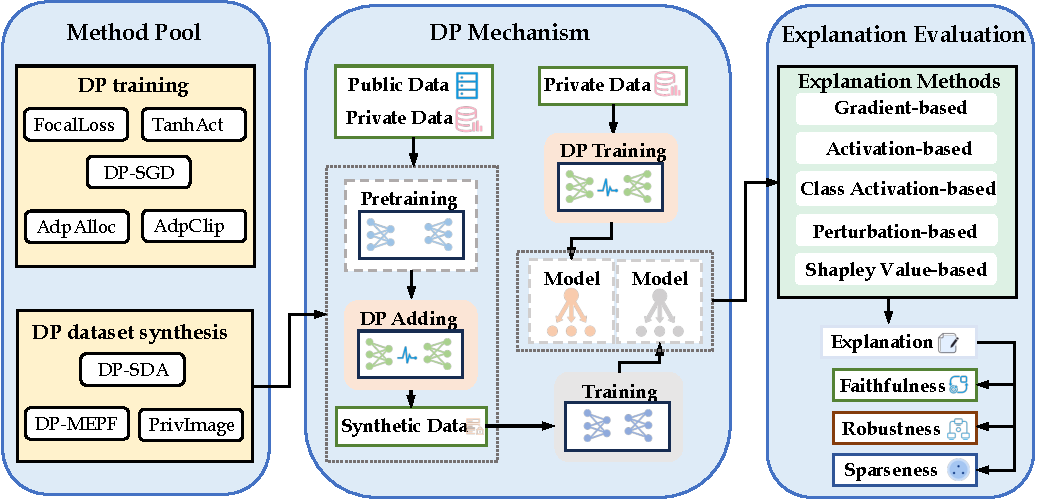
\includegraphics[width=\linewidth]{image/pipeline.pdf}
  \caption{Architectural overview of DPMI for assessing the impact of DP on model explainability. The system comprises three main modules: Method Pool, DP Mechanism, and Explanation Evaluation.}
  \label{fig:pipeline}
\end{wrapfigure}

\section{DPMI: System Design and Experimental Framework}
Our research framework investigates the interplay between DP and model explainability through a modular experimental design. Figure~\ref{fig:pipeline} presents the architectural overview of our evaluation system, which consists of three primary modules: (1) Method Pool, (2) DP Mechanism, (3) Explanation Evaluation. We detail each component within the overall system as follows.

\noindent \textbf{Method Pool. }
The foundation of our framework begins with the selection of DP machine learning approaches. We use two distinct methodological categories: DP training and DP dataset synthesis methods. Our selection of methods is guided by two key considerations: representing the full spectrum of state-of-the-art DP approaches and prioritizing diverse technical innovations. Detailed descriptions of these methods are provided in the Appendix~\ref{app:method_selection}.




% DP training (DPSGD~\cite{abadi2016deep} and its improvements: TanhAct~\cite{papernot2021tempered}, FocalLoss~\cite{shamsabadi2023losing}, AdpClip~\cite{andrew2021differentially}, and AdpAlloc~\cite{yu2019differentially}) and DP dataset synthesis methods (DPSDA~\cite{lin2023differentially}, Privimage~\cite{li2023meticulously}, and DP-MEPF~\cite{harder2022pre}).Our selection of methods is guided by two key considerations: representing the full spectrum of state-of-the-art differential privacy approaches and prioritizing diverse technical innovations. Detailed descriptions of these methods are provided in the Appendix~\ref{app:method_selection}.


\noindent \textbf{DP Mechanism. }
For DP training, this module directly utilizes private data and DP techniques to train a classification model.
For DP dataset synthesis methods, this module generates privacy-preserved synthetic data through a two-phase process of pre-training and privacy-focused fine-tuning. The synthetic data is then used to train classifiers using standard training methods.



\noindent \textbf{Explanation Evaluation. }
This module implements ten explainability algorithms through both the Captum library and custom implementations based on research papers, generating comprehensive attribution maps and visualizations that are evaluated across privacy-varying models using ROAD~\cite{rong2022consistent} (faithfulness), RIS~\cite{agarwal2022rethinking} (robustness), and Gini Index~\cite{chalasani2020concise} (sparseness) metrics. 
This selection enables comprehensive evaluations of DP's impact on model explainability across various dimensions. Detailed descriptions of these methods are provided in the Appendix~\ref{app:xai_method_selection} and ~\ref{app:eva_method_selection}.





% \noindent \textbf{Comparative Analysis.} The final module integrates results from previous components to deliver comprehensive insights into the relationship between differential privacy and model explainability. Our analysis framework examines this relationship through a systematic progression of experiments:

Through this system design, our framework enables comprehensive evaluation of the relationship between differential privacy and model explainability. We conduct a systematic progression of experiments that analyze how different DP implementations affect explainability metrics across various model architectures, datasets, and privacy settings, providing researchers and practitioners with actionable insights into privacy-explainability tradeoffs.

\section{Evaluations}\label{sec:evaluations}

\subsection{Evaluations Setup}
% For our experiments, we investigate multiple model architectures (ResNet20, WideResNet, and SimpleNN) across four standard image classification datasets (MNIST, FashionMNIST, CIFAR-10, and SVHN). We primarily use a privacy budget of $\varepsilon = 4$ with $\delta = 10^{-5}$ in our comparative analyses, while exploring various privacy budgets ranging from $\varepsilon \in \{0.2, 0.4, 0.8, 1, 4, 8, 10\}$ when examining privacy-utility trade-offs. We also investigate different gradient clipping thresholds $C \in \{4, 6, 8, 10\}$ to understand their impact on model explainability. 
Our experiments are conducted on four standard image classification datasets (MNIST, FashionMNIST, CIFAR-10, SVHN) using three model architectures: ResNet20, WideResNet, and SimpleNN. The primary experiments adopted a privacy budget of $\epsilon = 4$ ($\delta = 10^{-5}$), with additional exploration of privacy-utility tradeoffs across $\epsilon \in \{0.2, 0.4, 0.8, 1, 4, 8, 10\}$. Furthermore, we systematically analyzed the impact of the gradient clipping threshold $C \in \{4, 6, 8, 10\}$ on model explainability.
All experiments utilize Rényi DP for privacy accounting, with appropriate noise scales computed numerically. Detailed experimental configurations, including specific hyperparameters, model architecture adaptations, and dataset preprocessing, are provided in Appendix~\ref{app:exp_config}.

In assessment, we select one representative metric from each category. ROAD (Remove And Debias) evaluates faithfulness by ranking features according to their importance, progressively removing these features, and assessing the model's prediction accuracy after removal. A faster decrease in accuracy as the percentage of removed pixels increases indicates higher fidelity of the explanation. RIS (Relative Input Stability) measures robustness by comparing the relative change in explanations to the relative change in inputs:
\[
\text{RIS}(\mathbf{x}, \mathbf{x}', \mathbf{e}_\mathbf{x}, \mathbf{e}_{\mathbf{x}'}) = \max_{\mathbf{x}'} \frac{\left\|\frac{(\mathbf{e}_\mathbf{x} - \mathbf{e}_{\mathbf{x}'})}{\mathbf{e}_\mathbf{x}}\right\|_p}{\max(\left\|\frac{(\mathbf{x}-\mathbf{x}')}{\mathbf{x}}\right\|_p, \epsilon_{\min})}, \
\]
\[
\quad \forall \mathbf{x}' \text{ s.t. } \mathbf{x}' \in \mathcal{N}_\mathbf{x}; \ \hat{y}_\mathbf{x} = \hat{y}_{\mathbf{x}'}
\]
where $\mathbf{x}$ is the original input, $\mathbf{x}'$ is a perturbed input, $\mathbf{e}_\mathbf{x}$ and $\mathbf{e}_{\mathbf{x}'}$ are their respective explanations, $\mathcal{N}_\mathbf{x}$ is the neighborhood of $\mathbf{x}$, $\hat{y}_\mathbf{x}$ and $\hat{y}_{\mathbf{x}'}$ are the predicted labels, $p$ denotes the norm, and $\epsilon_{\min}$ is a small constant to prevent division by zero. 

The Gini Index measures sparseness by quantifying the concentration of importance across features:
\[
\text{Gini}(e(x)) = 1 - 2\sum_{k=1}^d \frac{|e_{(k)}(x)|}{||e(x)||_1}\left(\frac{d-k+0.5}{d}\right)
\]
where $e_{(k)}(x)$ is the k-th element after sorting attribution values by magnitude, and $d$ is the vector dimension. These three metrics provide a comprehensive evaluation framework for assessing the impact of DP on model explainability across multiple dimensions of explanation quality.


Using the evaluation framework and metrics that we have proposed, we performed a set of detailed experiments to answer the three subsequent research questions (RQs).

\begin{itemize}[leftmargin=*]

% \item \textbf{RQ1:} How do different DP methods perform in terms of explainability?

\item \textbf{RQ1:} How does the stage of noise injection in differential privacy (training-time versus data synthesis-time) affect model explainability?

\item \textbf{RQ2:} How do privacy budgets and gradient clipping thresholds affect the explainability of the model after adding DP?

\item \textbf{RQ3:} How do model architectures and datasets affect the explainability after adding DP?

\end{itemize}

\subsection{DP Method Comparison (RQ1)}

\noindent \textbf{Experiment Design.} To answer RQ1, we fixed the privacy budget at $\epsilon = 4$ (which allows these methods to maintain good accuracy). The experiments were conducted using the ResNet20 model trained on the CIFAR-10 dataset.

\begin{table*}[htbp]
\centering
\caption{Faithfulness, robustness, and sparseness scores across different DP and explanation methods. Bold font indicates the highest score in each column. In each table, the first five methods above the horizontal line are DP training methods, while the remaining methods are DP synthesis methods. We show the mean $\pm$ standard deviation of the performance averaged over five repeat experiments.}
\label{table:main}

% Faithfulness 子表
\subfloat[Faithfulness scores\label{table:faithfulness}]{%
\setlength{\tabcolsep}{2pt}%
\resizebox{1.0\textwidth}{!}{%
\begin{tabular}{l|*{5}{cc}}
\toprule
 & \multicolumn{2}{c}{Gradient-based} & \multicolumn{2}{c}{Perturbation-based} & \multicolumn{2}{c}{Shapley value-based} & \multicolumn{2}{c}{Activation-based} & \multicolumn{2}{c}{Class activation-based} \\
\cmidrule(lr){2-3} \cmidrule(lr){4-5} \cmidrule(lr){6-7} \cmidrule(lr){8-9} \cmidrule(lr){10-11}
 Methods & InputXGrad & FovEx & FeatureAblation & Occlusion & GradientShap & KernelShap & Activation & GradXActivation & GradCam & GradCamPlusScore \\
\midrule
\rowcolor[gray]{0.9}
Normal & 0.479 ±0.020 & 0.433 ±0.021 & 0.521 ±0.029 & 0.499 ±0.021 & 0.509 ±0.038 & 0.143 ±0.019 & 0.477 ±0.024 & 0.488 ±0.017 & 0.521 ±0.025 & 0.401 ±0.015 \\
DP-SGD & 0.257 ±0.016 & 0.394 ±0.020 & 0.308 ±0.037 & 0.398 ±0.031 & 0.277 ±0.046 & 0.149 ±0.027 & 0.424 ±0.022 & 0.395 ±0.024 & 0.390 ±0.022 & 0.330 ±0.021 \\
AdpAlloc & 0.358 ±0.017 & 0.340 ±0.022 & 0.332 ±0.027 & 0.326 ±0.014 & 0.323 ±0.011 & 0.109 ±0.026 & 0.323 ±0.027 & 0.288 ±0.025 & 0.289 ±0.026 & 0.328 ±0.020 \\
AdpClip & 0.333 ±0.023 & 0.414 ±0.027 & 0.388 ±0.030 & 0.450 ±0.034 & 0.347 ±0.039 & 0.102 ±0.022 & 0.378 ±0.019 & 0.295 ±0.023 & 0.302 ±0.024 & 0.349 ±0.015 \\
FocalLoss & 0.330 ±0.037 & 0.407 ±0.017 & 0.361 ±0.034 & 0.388 ±0.025 & 0.328 ±0.033 & 0.118 ±0.037 & 0.397 ±0.031 & 0.365 ±0.029 & 0.379 ±0.026 & 0.328 ±0.028 \\
TanhAct & 0.315 ±0.029 & 0.285 ±0.036 & 0.381 ±0.033 & 0.326 ±0.037 & 0.334 ±0.039 & 0.123 ±0.018 & 0.205 ±0.017 & 0.318 ±0.021 & 0.320 ±0.025 & 0.244 ±0.030 \\
\hline
DPSDA & 0.362 ±0.012 & 0.390 ±0.041 & 0.421 ±0.025 & 0.530 ±0.024 & 0.345 ±0.034 & 0.133 ±0.032 & 0.392 ±0.028 & 0.366 ±0.031 & 0.362 ±0.028 & 0.280 ±0.026 \\
DPMEPF & 0.316 ±0.028 & 0.428 ±0.030 & 0.261 ±0.013 & 0.377 ±0.017 & 0.328 ±0.014 & 0.192 ±0.027 & 0.342 ±0.015 & 0.337 ±0.018 & 0.296 ±0.015 & 0.355 ±0.022 \\
Privimage & \textbf{\underline{0.643}} ±0.035 & \textbf{\underline{0.527}} ±0.042 & \textbf{\underline{0.629}} ±0.031 & \textbf{\underline{0.537}} ±0.027 & \textbf{\underline{0.632}} ±0.019 & \textbf{\underline{0.612}} ±0.030 & \textbf{\underline{0.575}} ±0.035 & \textbf{\underline{0.494}} ±0.022 & \textbf{\underline{0.504}} ±0.039 & \textbf{\underline{0.444}} ±0.029 \\
\bottomrule
\end{tabular}%
}}

% Robustness 子表
\subfloat[Robustness scores\label{table:robustness}]{%
\setlength{\tabcolsep}{2pt}%
\resizebox{1.0\textwidth}{!}{%
\begin{tabular}{l|*{5}{cc}}
\toprule
 & \multicolumn{2}{c}{Gradient-based} & \multicolumn{2}{c}{Perturbation-based} & \multicolumn{2}{c}{Shapley value-based} & \multicolumn{2}{c}{Activation-based} & \multicolumn{2}{c}{Class activation-based} \\
\cmidrule(lr){2-3} \cmidrule(lr){4-5} \cmidrule(lr){6-7} \cmidrule(lr){8-9} \cmidrule(lr){10-11}
 Methods & InputXGrad & FovEx & FeatureAblation & Occlusion & GradientShap & KernelShap & Activation & GradXActivation & GradCam & GradCamPlusScore \\
\midrule
\rowcolor[gray]{0.9}
Normal & -3.44±0.11 & -6.69±0.52 & -2.82±0.10 & -2.49±0.17 & -5.61±0.28 & -5.06±0.18 & 5.21±0.24 & 2.05±0.27 & 2.00±0.16 & \underline{2.16}±0.28 \\
DP-SGD & -3.54±0.17 & -6.74±0.57 & -2.97±0.11 & -1.99±0.13 & -5.84±0.24 & -4.76±0.17 & 5.60±0.22 & 2.55±0.24 & 2.55±0.17 & \textbf{1.31}±0.29 \\
AdpAlloc & -3.45±0.24 & -5.48±0.55 & -2.84±0.14 & -2.37±0.14 & -6.04±0.27 & -4.76±0.14 & 5.75±0.28 & 2.17±0.29 & 2.20±0.15 & 0.31±0.25 \\
AdpClip & -3.37±0.15 & \textbf{\underline{-3.55}}±0.58 & -2.84±0.16 & -2.32±0.12 & -5.77±0.19 & -4.70±0.19 & 5.81±0.17 & 2.02±0.16 & 2.08±0.14 & 2.16±0.18 \\
FocalLoss & -3.29±0.22 & -6.17±0.63 & -2.91±0.12 & -2.39±0.19 & -5.72±0.17 & -4.85±0.13 & 5.52±0.23 & 2.42±0.32 & 2.38±0.15 & 2.08±0.21 \\
TanhAct & \textbf{\underline{-3.01}}±0.13 & -7.38±0.51 & -2.98±0.15 & -2.55±0.15 & -5.92±0.25 & -4.70±0.16 & 0.27±0.31 & 2.17±0.21 & 2.13±0.19 & -4.74±0.36 \\
\hline
DPSDA & -3.28±0.27 & -4.10±0.61 & \textbf{\underline{-2.50}}±0.18 & \textbf{\underline{-1.83}}±0.14 & -5.90±0.25 & -4.88±0.21 & \textbf{\underline{5.89}}±0.30 & 2.51±0.18 & 2.49±0.24 & -0.31±0.29 \\
DPMEPF & -3.44±0.34 & -6.51±0.53 & -2.99±0.11 & -1.78±0.22 & \textbf{\underline{-5.49}}±0.33 & -5.17±0.23 & 5.50±0.26 & \textbf{\underline{2.65}}±0.30 & \textbf{\underline{2.77}}±0.38 & -1.71±0.27 \\
Privimage & -3.57±0.37 & -9.27±0.68 & -3.30±0.27 & -2.72±0.19 & -5.75±0.18 & \textbf{\underline{-4.46}}±0.15 & 4.52±0.19 & 1.28±0.25 & 1.23±0.22 & -2.52±0.33 \\
\bottomrule
\end{tabular}%
}}

% Sparseness 子表
\subfloat[Sparseness scores\label{table:sparseness}]{%
\setlength{\tabcolsep}{2pt}%
\resizebox{1.0\textwidth}{!}{%
\begin{tabular}{l|*{5}{cc}}
\toprule
 & \multicolumn{2}{c}{Gradient-based} & \multicolumn{2}{c}{Perturbation-based} & \multicolumn{2}{c}{Shapley value-based} & \multicolumn{2}{c}{Activation-based} & \multicolumn{2}{c}{Class activation-based} \\
\cmidrule(lr){2-3} \cmidrule(lr){4-5} \cmidrule(lr){6-7} \cmidrule(lr){8-9} \cmidrule(lr){10-11}
 Methods & InputXGrad & FovEx & FeatureAblation & Occlusion & GradientShap & KernelShap & Activation & GradXActivation & GradCam & GradCamPlusScore \\
\midrule
\rowcolor[gray]{0.9}
Normal & 0.554±0.041 & 0.698±0.073 & 0.547±0.023 & 0.478±0.055 & 0.553±0.034 & 0.589±0.076 & 0.239±0.034 & \underline{0.459}±0.074 & \underline{0.470}±0.081 & \underline{0.470}±0.082 \\
DP-SGD & 0.543±0.052 & 0.718±0.069 & 0.536±0.024 & 0.464±0.059 & 0.545±0.037 & 0.539±0.066 & 0.173±0.012 & 0.385±0.065 & 0.374±0.077 & 0.270±0.070 \\
AdpAlloc & 0.544±0.055 & 0.707±0.072 & 0.543±0.025 & 0.486±0.062 & 0.539±0.042 & 0.538±0.073 & 0.199±0.033 & 0.415±0.057 & 0.420±0.069 & 0.355±0.071 \\
AdpClip & 0.548±0.061 & 0.706±0.070 & 0.541±0.024 & 0.468±0.057 & 0.547±0.040 & 0.551±0.074 & 0.204±0.025 & 0.416±0.043 & 0.419±0.067 & 0.264±0.089 \\
FocalLoss & 0.536±0.069 & 0.704±0.068 & 0.533±0.027 & 0.459±0.064 & 0.531±0.040 & 0.545±0.077 & 0.197±0.017 & 0.393±0.053 & 0.385±0.069 & 0.279±0.083 \\
TanhAct & 0.519±0.059 & 0.722±0.067 & 0.525±0.023 & 0.438±0.049 & 0.519±0.030 & \textbf{\underline{0.643}}±0.096 & \textbf{\underline{0.409}}±0.013 & 0.294±0.061 & 0.286±0.082 & \textbf{0.444}±0.062 \\
\hline
DPSDA & 0.598±0.050 & 0.724±0.071 & \textbf{\underline{0.587}}±0.029 & \textbf{\underline{0.504}}±0.065 & \textbf{\underline{0.607}}±0.038 & 0.532±0.061 & 0.163±0.031 & \textbf{0.429}±0.058 & \textbf{0.431}±0.072 & 0.323±0.073 \\
DPMEPF & 0.540±0.057 & \textbf{\underline{0.733}}±0.078 & 0.550±0.023 & 0.434±0.043 & 0.539±0.029 & 0.605±0.067 & 0.155±0.026 & 0.356±0.049 & 0.367±0.066 & 0.256±0.049 \\
Privimage & \textbf{\underline{0.610}}±0.067 & 0.699±0.082 & 0.559±0.031 & 0.484±0.042 & 0.605±0.045 & 0.557±0.088 & 0.149±0.035 & 0.388±0.068 & 0.401±0.085 & 0.395±0.067 \\
\bottomrule
\end{tabular}%
}}
\end{table*}

\noindent \textbf{Result Analysis.}
Table~\ref{table:faithfulness}-\ref{table:sparseness} present a comprehensive comparison of these DP methods across various explainability metrics and techniques. It's important to note that some of the data in this table are derived from processed values before calculating the mean and standard deviation. Specifically, the robustness values are presented as negative logarithms, while the faithfulness scores are calculated as 1 minus the normalized area under the curve ratio. The analysis of this processed data reveals performance differences among DP methods:

% Tables~\ref{table:faithfulness}-\ref{table:sparseness} comprehensively compare various explainability metrics of different DP methods. Notably, some metrics involve preprocessed data: robustness values are displayed as negative logarithms, while faithfulness scores derive from the formula $1 - \text{normalized area under the curve ratio}$. Analysis reveals significant performance disparities among DP methods. The analysis of this processed data reveals performance differences among DP methods:

\begin{tcolorbox}[colback=gray!20, colframe=gray!20, boxrule=0pt, arc=0pt, left=5pt, right=5pt, top=5pt, bottom=5pt]
\noindent \textbf{PrivImage successfully balances privacy and faithfulness of explainability.} PrivImage's superiority can be attributed to its innovative two-phase training framework: First, pre-training on public data establishes stable gradient patterns for core semantic features; second, DP-SGD fine-tuning preserves these patterns through controlled noise injection. This approach fundamentally addresses the limitations of conventional methods by maintaining model explainability while ensuring privacy guarantees.
\end{tcolorbox}

Standard DP-SGD severely degrades gradient-based explainability methods due to unmodulated noise and fixed gradient clipping, while activation/class activation-based approaches show stronger robustness, possibly because leveraging activation values for explainability mitigates the impact of noise addition and gradient clipping. This suggests that despite gradient perturbations, feature hierarchies remain partially intact.

Adaptive mechanisms show varying effectiveness depending on the explainability methods. AdpClip~\cite{andrew2021differentially}, which adjusts gradient clipping strategies, outperforms DP-SGD in gradient-based and perturbation-based methods, but performs worse in activation-based methods. Meanwhile, AdpAlloc demonstrates modest advantages in certain gradient-based methods compared to standard DP-SGD. The Tanh activation function often performs poorly in most explanation techniques because its limited output range leads to gradient saturation, hiding important features.

\noindent \textbf{DP dataset synthesis methods vary in how they affect explainability robustness. }Model trained with DPSDA demonstrates better robustness across most explainability methods compared to normal model, while model trained with PrivImage shows worse explainability robustness than normal model. This difference may be due to the fact that, compared to PrivImage, DPSDA makes the synthesized data semantically consistent with the original training data distribution, which facilitates higher robustness.

DPSGD exhibits varied robustness across explainability methods.
It shows poorer robustness than normal models in gradient-based explainability methods, but superior robustness in activation-based and class activation-based methods. DPSGD's noise injection disrupts gradient landscapes, causing poor performance in gradient-based explainability methods. However, this same noise acts as regularization for activation-based methods, preventing overfitting to specific features and creating more robust internal representations that distribute attention more evenly across relevant input regions, resulting in improved robustness for activation and class activation-based explainability techniques.

\noindent \textbf{Differential privacy methods weaken the interpretive simplicity of a model.} Most models that add differential privacy are less concise than regular models, and the gap between different explainability methods is significant. In scenarios where simplicity is important, it is recommended to use a high-performing interpretable method such as FovEx.

\subsection{Parameter Sensitivity of DP Methods (RQ2)}
\noindent \textbf{Experiment Design.}
We conducted experiments with varying privacy budgets ($\epsilon = \{0.2, 0.4, 0.8, 1.0, 4.0, 8.0, 10.0\}$) across different differential privacy methods. We further evaluate the faithfulness of DP-SGD models with varrying gradient clipping values ($C = 4.0, 6.0, 8.0, 10.0$) under a certain privacy budget $\epsilon = 10$. 

\noindent \textbf{Result Analysis.} In summary, the main findings of this section can be outlined as follows:

\begin{wrapfigure}{l}{0.5\textwidth} 
  \centering
  \vspace{0pt}
  \includegraphics[width=\linewidth]{1_dif_epsilon.pdf}
  \caption{Mean faithfulness comparison across $\epsilon$ values for explainability methods. The black dashed line indicates the faithfulness score of the normal model, while the blue dashed line corresponds to the score of the model with gradient clipping alone. }
  \label{fig:epsilon_comparison}
\end{wrapfigure}

\noindent \textbf{The link between privacy budget and model explainability faithfulness is nonlinear, with PrivImage maintaining the highest faithfulness across all budgets. }Figure~\ref{fig:epsilon_comparison} (a) presents the faithfulness scores of various differential privacy methods under different privacy budgets. Models trained with DPSGD demonstrate higher faithfulness at larger privacy budgets, yet models with gradient clipping alone do not exhibit the highest faithfulness scores. Both DPSDA and PrivImage show their lowest faithfulness at $\epsilon=4$ and highest at $\epsilon=8$, while DPMEPF demonstrates less significant variation across privacy budgets compared to the other three methods. Notably, PrivImage achieves superior faithfulness performance across all $\epsilon$ values, consistently outperforming the normal model.

Figure~\ref{fig:epsilon_comparison} (b) presents the faithfulness scores of various differential privacy methods under different privacy budgets (lower). Interestingly, models trained with PrivImage-generated data show a pattern where explainability faithfulness decreases as privacy budget increases within this lower range, while maintaining excellent faithfulness scores across the entire low privacy budget interval. This suggests that PrivImage is a superior choice in scenarios requiring strict privacy budget limitations, as its two-phase training approach preserves more data characteristics beneficial for explainability.

Under low $\epsilon$, DP dataset synthesis yields more faithful explainability than DP training. Besides PrivImage, both DPSDA and DPMEPF outperform DPSGD under low privacy budgets, likely because DP dataset synthesis methods add noise during data generation rather than directly to gradients. This noise addition approach avoids direct interference with model gradient computations, resulting in less impact on model explainability. At extremely low privacy budgets ($\epsilon=0.2$), only models trained on data generated by PrivImage and DPSDA maintain usable levels of explainability faithfulness, capable of providing relatively reliable explanations for model decisions.

\begin{tcolorbox}[colback=gray!20, colframe=gray!20, boxrule=0pt, arc=0pt, left=5pt, right=5pt, top=5pt, bottom=5pt]
\noindent \textbf{Gradient clipping degrades DPSGD faithfulness vs normal models.} Figure~\ref{fig:clipping_comparison} shows the percentage decrease in explainability faithfulness for models with only gradient clipping compared to normal models. Even without adding noise, the model's faithfulness exhibits a notable decline, likely because gradient clipping limits the magnitude of parameter updates, disrupting the natural learning process and making it difficult for explainability methods to obtain feature relationships.
\end{tcolorbox}

\begin{figure}[!h]
\begin{minipage}[t]{0.48\columnwidth}
  \vspace{0pt} % 确保顶部对齐参考点一致
  \includegraphics[width=\linewidth]{2_norm_clip.pdf}
  \caption{Faithfulness Comparison: Normal vs. Gradient Clipping-only Models. Percentage atop bars indicates faithfulness decline vs. normal.}
  \label{fig:clipping_comparison}
\end{minipage}
\hfill
\begin{minipage}[t]{0.48\columnwidth}
  \vspace{0pt} % 确保顶部对齐参考点一致
  \includegraphics[width=\linewidth]{3_clip_value_comparison.pdf}
  \caption{Effect of Gradient Clipping Threshold on Interpretation Faithfulness. Most methods peak at 8.0.}
  \label{fig:clipping_threshold}
\end{minipage}
\end{figure}

Moderate gradient clipping thresholds can lead to relatively good model explainability. Figure~\ref{fig:clipping_threshold} shows how the faithfulness of models trained with DPSGD on different explainability methods varies with the gradient clipping threshold. As the gradient clipping threshold increases, the faithfulness of most explainability methods first increases and then decreases, reaching the highest faithfulness when $C = 8.0$. This bell - shaped relationship between the clipping threshold and faithfulness can be attributed to two conflicting mechanisms: When the threshold is too low, excessive gradient constraint restricts the model's capacity to learn meaningful feature relationships. When the threshold is too high, uncontrolled gradient updates may cause unstable training and less interpretable representations. These findings offer practical insights for implementing DPSGD methods: although the selection of the privacy budget may mainly be guided by privacy requirements, carefully adjusting the gradient clipping threshold is essential for maintaining model explainability.

\subsection{Model Architecture and Dataset Comparison (RQ3)}

\noindent \textbf{Experiment Design.}
We conducted experiments using three neural architectures (ResNet20, WideResNet, SimpleNN) trained with identical privacy parameters (privacy budget ($\epsilon=4$) and gradient clipping threshold $C=4$) across four differential privacy methods: DPSGD, DPSDA, DPMEPF, and PrivImage. For ResNet20 with DPSGD, we tested on CIFAR-10, MNIST, FMNIST, and SVHN datasets, performing explainability analysis via GradCam($\varepsilon = 10$, and $C=4$ ). 

\noindent \textbf{Result Analysis.}Figures~\ref{fig:architectures} and~\ref{fig:datasets-comparison} reveal the comparative performance of explainability methods across neural architectures and datasets, respectively. Based on these visualizations, we summarize the key findings below:

\noindent \textbf{Methods with superior explainability faithfulness excel on complex architectures. }Data generated by PrivImage demonstrates higher explainability faithfulness when used with WideResNet. This may be because models trained on PrivImage-generated data have better explainability faithfulness overall, enabling them to capture the rich information in more complex models and produce explanations with higher faithfulness.

DPSGD's explainability faithfulness varies by model architecture and method type. DPSGD shows better faithfulness on SimpleNN for gradient or perturbation-based explainability methods, while performing better on ResNet20 for activation-based explainability methods. This discrepancy likely stems from DPSGD's noise addition and gradient clipping operations affecting simpler and more complex architectures differently. In simpler networks like SimpleNN, gradient paths are more direct, making gradient-based methods more resilient to the bounded noise. However, in more complex architectures like ResNet20, the activation patterns benefit from the regularization effect of differential privacy, creating more robust internal representations.

\begin{figure*}[!t]
\centering
\includegraphics[width=\textwidth]{image/5_model_heatmaps.pdf}
% \caption{Comparison of Explainability Metrics Across Different Model Architecture.}
\caption{Comparison of explainability metrics across different Model architecture($\epsilon=4$). Faithfulness intensity is encoded in blue saturation, while robustness uses divergent red (positive) and blue (negative) hues with magnitude scaling.}
\label{fig:architectures}
\end{figure*}

DPSDA demonstrates good faithfulness performance on ResNet20. This is because ResNet20 provides the right balance for learning robust feature representations while preserving important structural relationships within the data that are critical for maintaining explainability faithfulness.

For robustness, DPSGD demonstrates better robustness on ResNet20, while DPSDA shows superior robustness on WideResNet. PrivImage performs well on SimpleNN, and DPMEPF displays more balanced performance across architectures. When selecting explainability methods, Activation, Grad×Activation, and GradCAM are good choices as they perform consistently well across all three model architectures and four DP methods.

\textbf{Digital-centric datasets (MNIST, SVHN) exhibit higher faithfulness metrics compared to object recognition datasets (FMNIST, CIFAR-10). }
MNIST achieves the highest model faithfulness, followed by SVHN, both significantly outperforming FMNIST (lowest) and CIFAR-10 (moderate). This is likely because digit-class datasets have simpler representations with well-defined structural patterns (e.g., stroke connectivity, spatial regularity), enabling precise localization of causally important features. In contrast, object-class datasets involve complex variations (e.g., viewpoint diversity, texture ambiguity) that introduce noise in feature attribution.
% MNIST achieves the highest model faithfulness, followed by SVHN, both clearly outperforming FMNIST and CIFAR-10. This is mainly due to the structural simplicity and consistency of digit datasets. MNIST digits are monochrome, centered, and uniform, making it easier for models to learn focused and causally relevant features. SVHN, though based on natural images, still offers consistent layouts and strong local cues. In contrast, FMNIST and CIFAR-10 involve more visual complexity—such as varying shapes, textures, and backgrounds—which makes it harder for models and explanation methods to isolate truly important features, leading to lower faithfulness.

% CIFAR-10 demonstrates the best robustness across most methods, potentially due to its higher complexity as a multi-class object recognition dataset containing diverse categories, cluttered backgrounds, and real-world noise, which forces models to learn noise-resistant feature representations, thereby enhancing the stability and interference immunity of explanation results.

CIFAR-10 demonstrates the best robustness across most dp methods, a trend that can be understood by considering the dataset's inherent visual diversity and noise. As a multi-class object recognition dataset, CIFAR-10 contains highly heterogeneous classes with substantial intra-class variation and environmental distractions. These properties compel models to develop more invariant and generalizable features that are less sensitive to noise perturbations, including those introduced by differentially private training. 
\begin{figure*}[!t]
    \centering
    \includegraphics[width=\textwidth]
    {4_dataset.pdf}
    \caption{Comparison of faithfulness, robustness, and sparseness metrics across different datasets in DP Methods ($\epsilon=10$). }
    \label{fig:datasets-comparison}
\end{figure*}

% For sparseness, SVHN shows a clear advantage, likely attributed to its domain-specific properties: street view house numbers typically exhibit centralized digit layouts, high color contrast, and uniform character scales, allowing explanation methods to focus on compact discriminative regions with minimal sparse activation.

For sparseness, the SVHN dataset exhibits a distinct advantage, primarily due to the domain-specific visual characteristics of street view house numbers. The digits are typically well-centered, high in contrast, and standardized in scale, which naturally guides explanation methods to focus on tight, localized regions of interest. These properties reduce the spatial spread of salient feature maps, leading to higher sparseness scores. 

% From a theoretical perspective, such intrinsic structure in the data acts as an inductive bias that complements the objectives of explanation methods—namely, to isolate minimal and relevant features—thus resulting in compact activation maps even under privacy-preserving training regimes.


\section{Conclusion} \label{sec:conclusion_limitation}
This paper presents a systematic study of the impact of differential privacy (DP) on model explainability. We introduce the DPMI framework, integrating two categories of DP mechanisms and five explainability methods, to evaluate how DP affects explanation fidelity. Our findings reveal that DP significantly influences explainability. DP data synthesis methods consistently preserve explanation faithfulness better than in-training noise injection approaches. Within DP-SGD, gradient clipping affects explainability more than noise addition, with optimal clipping thresholds balancing utility and privacy. We further observe that model architecture mediates this trade-off: wider networks favor DP data synthesis, while simpler models yield more faithful explanations under DP training. These insights inform the selection of DP techniques when explainability is a critical requirement.



% This paper comprehensively investigates the relationship between DP and model explainability, addressing the critical challenge of balancing privacy protection with explainability in ML systems. Through systematic evaluation of diverse privacy approaches and explainability methods, we have identified several key insights that advance our understanding of this important trade-off.

% Our analysis reveals that generative privacy methods, particularly PrivImage, consistently outperform gradient-perturbation approaches in maintaining explanation faithfulness while preserving privacy guarantees. This superiority stems from PrivImage's two-phase training framework that establishes stable gradient patterns for core semantic features through public data pre-training before applying controlled noise injection during DP-SGD fine-tuning. This approach addresses the limitations of conventional methods by preserving model explainability under DP.

% We show that gradient clipping significantly impacts model explainability—often more substantially than noise addition—with faithfulness scores exhibiting a bell-shaped response to clipping thresholds. An optimal threshold range (around 6.0-8.0) balances between preserving model explainability and maintaining effective privacy protection, with excessive constraint limiting the model's ability to learn meaningful feature relationships and insufficient constraint leading to unstable training.

% Despite our comprehensive analysis, this work has limitations: our benchmark evaluations may not fully capture challenges in real-world deployment scenarios where adversarial attacks, model updates, and domain shifts could further complicate the privacy-explainability balance; additionally, our computational metrics for explanation quality might not perfectly align with human perception and understanding, highlighting the need for domain expert evaluation in future work.


% \section*{References}
% \section*{References}
\bibliographystyle{plain}  % You can use other styles like 'unsrt', 'alpha', etc.
\bibliography{references}   % This references your references.bib file


% References follow the acknowledgments in the camera-ready paper. Use unnumbered first-level heading for
% the references. Any choice of citation style is acceptable as long as you are
% consistent. It is permissible to reduce the font size to \verb+small+ (9 point)
% when listing the references.
% Note that the Reference section does not count towards the page limit.
% \medskip


% {
% \small


% [1] Alexander, J.A.\ \& Mozer, M.C.\ (1995) Template-based algorithms for
% connectionist rule extraction. In G.\ Tesauro, D.S.\ Touretzky and T.K.\ Leen
% (eds.), {\it Advances in Neural Information Processing Systems 7},
% pp.\ 609--616. Cambridge, MA: MIT Press.


% [2] Bower, J.M.\ \& Beeman, D.\ (1995) {\it The Book of GENESIS: Exploring
%   Realistic Neural Models with the GEneral NEural SImulation System.}  New York:
% TELOS/Springer--Verlag.


% [3] Hasselmo, M.E., Schnell, E.\ \& Barkai, E.\ (1995) Dynamics of learning and
% recall at excitatory recurrent synapses and cholinergic modulation in rat
% hippocampal region CA3. {\it Journal of Neuroscience} {\bf 15}(7):5249-5262.
% }


%%%%%%%%%%%%%%%%%%%%%%%%%%%%%%%%%%%%%%%%%%%%%%%%%%%%%%%%%%%%

\appendix

\section{Appendix}

\subsection{Related Work}\label{app:related_work}

\subsubsection{Differential Privacy}
Differential Privacy (DP) provides a mathematical framework for quantifying and limiting privacy leakage in machine learning models~\cite{abadi2016deep}. Abadi et al. ~\cite{abadi2016deep} first introduced DP-SGD, which incorporates gradient clipping and noise addition to achieve formal privacy guarantees during training. Subsequent works improve the privacy-utility trade-off through architectural modifications~\cite{papernot2021tempered}, specialized loss functions ~\cite{shamsabadi2023losing}, and adaptive privacy parameter adjustment ~\cite{andrew2021differentially,yu2019differentially}. Another line of research focuses on differentially private synthetic data generation~\cite{gong2025dpimagebench}, which separates the privacy mechanism from downstream model training while preserving data utility.


\subsubsection{explainability Methods}
explainability methods aim to reveal how neural networks make decisions by highlighting influential input features~\cite{zhang2021survey,fan2021interpretability,dong2017improving,salahuddin2022transparency,li2022interpretable,linardatos2020explainable,ghorbani2019interpretation}. These methods can be categorized into five main classes based on their underlying principles and mechanisms. Gradient-based methods utilize model gradients to attribute importance to input features~\cite{simonyan2014deepinsideconvolutionalnetworks,panda2024human,zeiler2013visualizingunderstandingconvolutionalnetworks,dhamdhere2018importantneuron,leino2018influencedirectedexplanationsdeepconvolutional}. Activation-based methods analyze internal network activations to understand model behavior~\cite{li2021deep}. Class activation-based methods generate visual explanations by highlighting discriminative regions for specific classes~\cite{zhou2016learning,selvaraju2017grad,chattopadhay2018grad,wang2020score,soomro2024grad++}. Perturbation-based methods examine how model outputs change when inputs are systematically modified~\cite{zeiler2013visualizingunderstandingconvolutionalnetworks,ribeiro2016whyitrustyou}. Shapley value-based methods apply game theory concepts to fairly distribute prediction credits among features~\cite{castro2009polynomial,lundberg2017unified}.

\subsubsection{Evaluation of explainability}
Evaluating explainability methods requires assessing multiple dimensions of explanation quality~\cite{zhou2021evaluating,nguyen2020quantitative,carvalho2019machine,gilpin2018explaining}. Faithfulness measures how accurately explanations reflect model behavior~\cite{rong2022consistent,lyu2024towards,dasgupta2022framework}. Robustness evaluates explanation stability under input perturbations~\cite{agarwal2022rethinking,hsieh2020evaluations}. Sparseness measures how concisely explanations identify important features~\cite{chalasani2020concise}.

\subsection{Taxonomy and Methodology}
This section provides an overview of our taxonomy, categorying the selected DP algorithms and explainability methods. 

\subsubsection{Differential Privacy Methods}\label{app:method_selection}

Recent advancements in DP implementation for machine learning models can be broadly categorized into two main types: DP training~\cite{wei2023dpmlbench} and DP dataset synthesis.~\cite{gong2025dpimagebench}

\noindent \textbf{DP training.} DP-SGD~\cite{abadi2016deep} is widely used to train the machine learning model under DP constriant~\cite{dwork2008differential}. It operates by sampling a batch of data points, computing individual gradients for each sample, clipping these gradients to bound their sensitivity, averaging the clipped gradients, adding calibrated Gaussian noise, and finally using the resulting noisy gradient to update model parameters.

While the vanilla DP-SGD~\cite{abadi2016deep} algorithm establishes fundamental privacy protection, it often comes with utility trade-offs that have prompted the research community to develop various enhanced approaches aimed at minimizing performance degradation while maintaining privacy guarantees~\cite{valdez2019users}. These methods modify the training process through three mechanisms: 
\begin{itemize}[leftmargin=*]
\item Model architecture adaptations form the first pillar, exemplified by techniques like \textit{TanhAct~\cite{papernot2021tempered}} that substitute conventional ReLU activations with tanh functions. This architectural shift improves numerical stability when applying noise injection during training.

\item Loss function specialization constitutes the second mechanism. Methods such as \textit{FocalLoss~\cite{shamsabadi2023losing}} redesign the optimization landscape by assigning higher weights to misclassified examples, simultaneously addressing model utility and gradient sensitivity under privacy constraints.

\item Gradient processing pipelines complete the framework through enhancements to DP-SGD~\cite{abadi2016deep} primitives: 
(i) \textit{AdpClip~\cite{andrew2021differentially}} dynamically tunes gradient clipping thresholds using real-time norm statistics; 
(ii) Noise injection strategies like \textit{RGP(Rényi Gradient Perturbation)~\cite{yu2021large}} and \textit{GGP(Gaussian Gradient Perturbation)~\cite{yu2021not}} implement refined sampling distributions; 
(iii) \textit{AdpAlloc~\cite{yu2019differentially}} optimizes the $\epsilon$-budget allocation across training phases via adaptive scheduling.
\end{itemize}

\noindent \textbf{DP dataset synthesis.}
These methods focus on creating synthetic datasets that preserve privacy while maintaining utility:

\begin{itemize}[leftmargin=*]

    \item \textit{DP-GAN} (Differentially Private Generative Adversarial Network)~\cite{xie2018differentially} addresses privacy concerns in GANs by introducing differential privacy guarantees through carefully designed noise addition to gradients during training. This approach prevents the learned generative distribution from concentrating too heavily on training samples, which could otherwise reveal sensitive information from private datasets such as medical records. The method implements the differential privacy mechanism by clipping gradients to bound their sensitivity and then adding calibrated Gaussian noise to achieve $(\epsilon, \delta)$-differential privacy. 
    
    \item \textit{DPDM} (Differentially Private Diffusion Models)~\cite{dockhorn2022differentially} combines diffusion models with differential privacy principles to generate high-quality synthetic data while preserving privacy~\cite{majeed2023attribute}. This approach implements differentially private stochastic gradient descent (DP-SGD) and introduces noise multiplicity, a specialized modification of DP-SGD designed specifically for training diffusion models. DPDM achieves state-of-the-art performance on image generation benchmarks under privacy constraints. Notably~\cite{tsai2024differentially}, classifiers trained on DPDM-generated synthetic data demonstrate comparable performance to those trained directly with DP-SGD on original data, establishing a new benchmark for privacy-preserving synthetic data generation.

     \item \textit{DPSDA} (Differentially Private Synthetic Data with foundation model APIs)~\cite{lin2023differentially} employs a Private Evolution framework using iterative operations with random and mutation APIs. This approach allows private samples to guide the generation process and has achieved promising results on datasets like CIFAR10 with low privacy costs. DPSDA can leverage large foundation models for processing specialized images, offering advantages in deployment ease and cost-effectiveness~\cite{xu2024deploying}.
    
    \item \textit{DP-MERF} (Differentially-Private Mean Embeddings with Random Features)~\cite{harder2021dp} leverages random feature representations of kernel mean embeddings to compare true and synthetic data distributions~\cite{muandet2017kernel}. By detaching data-dependent terms from synthetic data-dependent terms, it minimizes privacy costs during generative model training and eliminates sensitivity-related hyperparameter tuning through norm-bounded random features. 
    
    \item \textit{PDP-Diffusion} (Private Diffusion Pre-training)~\cite{ghalebikesabi2023differentially} leverages privately fine-tuned pre-trained diffusion models to generate high-quality synthetic data with privacy guarantees. By applying differential privacy techniques to ImageNet pre-trained diffusion models with over 80M parameters, this approach achieves state-of-the-art results on datasets like CIFAR-10 and Camelyon17 in terms of both FID scores and downstream classification accuracy. The method demonstrates that privately fine-tuned diffusion models can effectively bridge significant distribution shifts between pre-training and fine-tuning data, while maintaining privacy guarantees and generating unlimited synthetic samples for downstream tasks and hyperparameter optimization.
   
    \item \textit{DP-MEPF} (Differentially Private Maximum Entropy Perception Features)~\cite{harder2022pre} constructs kernel functions by learning perceptual features from public data. It utilizes a unique privatization approach that minimizes excessive noise during generator training. Experiments on datasets such as MNIST and CIFAR-10 demonstrate DP-MEPF~\cite{harder2022pre} capability to generate high-quality images with strong downstream task performance under relatively low privacy budgets.
    
    \item \textit{PrivImage~\cite{li2023meticulously}} establishes semantic query functions using public datasets to determine the semantic distribution of sensitive datasets. It selects similar semantic data from public datasets for pre-training, then pre-trains generative models using the selected data. The model is subsequently fine-tuned on sensitive datasets using DP-SGD\cite{abadi2016deep}. PrivImage\cite{li2023meticulously} effectively addresses challenges in existing differentially private image generation methods, particularly training instability and high computational resource requirements.
    
\end{itemize}


Our selection of methods is guided by two key considerations: representing the full spectrum of state-of-the-art differential privacy approaches and prioritizing diverse technical innovations. These innovations include gradient processing improvements (AdpClip~\cite{andrew2021differentially}, AdpAlloc~\cite{yu2019differentially}), architectural adaptations (TanhAct~\cite{papernot2021tempered}), loss function specializations (FocalLoss~\cite{shamsabadi2023losing}), and various generative frameworks. 

For our experiments, we select methods from both direct training modifications and synthetic data generation techniques. From DP training methods, we include AdpClip~\cite{andrew2021differentially}, AdpAlloc~\cite{yu2019differentially}, FocalLoss~\cite{shamsabadi2023losing}, TanhAct~\cite{papernot2021tempered}, and standard DP-SGD\cite{abadi2016deep}. From DP dataset synthesis methods, we incorporate DPSDA~\cite{lin2023differentially}, DP-MEPF~\cite{harder2022pre}, and PrivImage\cite{li2023meticulously}. This diversity allows us to comprehensively evaluate how different DP implementation strategies affect model explainability across various privacy-utility trade-offs while addressing practical challenges such as training instability, computational efficiency, and performance degradation.

\subsubsection{explainability Methods}\label{app:xai_method_selection}
explainability methods enhance the transparency of deep learning models by providing insights into their decision-making processes. In our analysis, we focus on post-hoc explainability methods, which can be applied after model training without requiring changes to the model architecture. These methods are particularly valuable for examining how privacy-preserving techniques affect model explanations.

Based on our comprehensive analysis of explainability approaches, we extend the traditional taxonomy that categorizes post-hoc explainability methods into three primary classes (internal representation analysis, perturbation-based, and Shapley value-based methods). Our refined framework further divides the internal representation analysis category into three distinct approaches:

\begin{itemize}[leftmargin=*]
\item \textsl{Gradient-based methods:} Focus on how model outputs change with respect to input features.

\item \textsl{Activation-based methods:} Analyze internal activation patterns within the network.

\item \textsl{Class activation-based methods:} Highlight regions in inputs that strongly activate class-specific features.

\end{itemize}






Together with the established perturbation-based and Shapley value-based methods, this creates a five-category classification system as shown in Table~\ref{tab:xai_methods}. The table summarizes various algorithms within each category and indicates their key characteristics: whether they use gradient information (Grad), activation values (Activ), layer-specific information (Layer), or class discriminative features (Class), as well as their explanation mechanism (Mech). This granular taxonomy enables thorough assessment of how different approaches illuminate various aspects of model behavior under privacy constraints, particularly when analyzing the distinct impacts of differential privacy methods (DP training through gradient/parameter perturbation and DP dataset synthesis through generative models) on model explainability while maintaining compatibility with the established three-class framework.


Based on this categorization system, the existing a posteriori explainability methods are described below:

\begin{itemize}[leftmargin=*]
    \item \textit{Gradient-based Methods.} 
\textit{Saliency~\cite{simonyan2014deepinsideconvolutionalnetworks}} computes input gradients, equivalent to the coefficients in a first-order Taylor expansion of the model at the input. The absolute values of these gradients represent feature importance.
    \textit{InputXGradient} computes feature importance by element-wise multiplication of input features with their corresponding gradients.
\textit{FovEx~\cite{panda2024human}} implements a biologically-inspired approach that focuses explanations on regions of high interest through a weighted combination of gradients and activations.
\textit{Deconvolution~\cite{zeiler2013visualizingunderstandingconvolutionalnetworks}} computes input gradients but override ReLU backpropagation to propagate only non-negative gradients. The former applies ReLU to input gradients, while the latter applies ReLU to output gradients. Though proposed for convolutional networks, both methods generalize to other architectures.
\textit{Integrated Gradients~\cite{sundararajan2017axiomatic}} computes the path integral of input gradients from a baseline to the input instance. The integral is typically approximated via Riemann sums or Gauss-Legendre quadrature.
\textit{Conductance~\cite{dhamdhere2018importantneuron}} integrates neuron activation values with both input-to-neuron and neuron-to-output partial derivatives to assess neuron importance comprehensively.
\textit{Internal Influence~\cite{leino2018influencedirectedexplanationsdeepconvolutional}} is a variant of Integrated Gradients~\cite{sundararajan2017axiomatic} that computes the path integral of layer gradients (instead of input gradients) from a baseline to the input instance.

\item \textit{Activation-based Methods.}
\textit{DeepLIFT~\cite{li2021deep}} is a backpropagation-based method that attributes input deviations by propagating differences between inputs and reference baselines through non-linear activations. It quantifies neuron contributions via "multipliers" to explain output differences relative to the reference.
\textit{GradientXActivation} enhances layer-wise attribution by combining activation values with their corresponding gradients.
    \textit{Activation} analyzes activation patterns at specific network layers to reveal internal representation characteristics.

    \item \textit{Class Activation-based Methods.}
    \textit{Class Activation Mapping (CAM)~\cite{zhou2016learning}} is a visualization technique that identifies discriminative regions in input images influencing convolutional neural network (CNN) predictions. Its core mechanism combines global average pooling (GAP) and linear layers to compute weighted sums of feature maps, generating class-specific activation heatmaps. 
    \textit{GradCam~\cite{selvaraju2017grad}} generates visual explanations by highlighting important regions using class-specific gradient information.
    \textit{Grad-CAM++~\cite{chattopadhay2018grad}} is an advanced gradient-based visual explanation method for convolutional neural networks (CNNs), designed to improve object localization and multi-instance explainability compared to Grad-CAM. By refining gradient weighting mechanisms, it addresses critical limitations in scenarios with multiple objects of the same class or fine-grained feature discrimination.  
    \textit{Score-CAM~\cite{wang2020score}} is a gradient-free visual explanation method for convolutional neural networks (CNNs) that leverages channel-wise forward activation scores to generate class-discriminative heatmaps. By eliminating gradient dependence, it addresses gradient saturation and noise sensitivity issues inherent in prior gradient-based CAM variants.  
\textit{GradCamPlusScore~\cite{soomro2024grad++}} combines GradCAM++~\cite{jamil2023advanced} and ScoreCAM~\cite{wang2020score} approaches to produce refined visual explanations with enhanced precision.

\begin{table}[!t]
\centering
\small
    \caption{Summary of Explainable AI Methods. ``\scalebox{1.5}{$\bullet$}'' means that the algorithm involves this property; ``\scalebox{1.5}{$\circ$}'' means that it does not. The table categorizes various explainability algorithms by whether they use gradient information (Grad), activation values (Activ), layer-specific information (Layer), or class discriminative features (Class), as well as their explanation mechanism (Mech). }

\label{tab:xai_methods}
\setlength{\tabcolsep}{6pt}  % 减小列间距
\begin{tabular}{l|lccccc}
\toprule
\textbf{Category} & \textbf{Algorithm} & \textbf{Grad.} & \textbf{Activ.} & \textbf{Layer} & \textbf{Class} & \textbf{Mech.} \\
\midrule
\multirow{7}{*}{\textbf{Gradient-based}} & Saliency~\cite{simonyan2014deepinsideconvolutionalnetworks} & \scalebox{1.5}{$\bullet$} & \scalebox{1.5}{$\circ$} & \scalebox{1.5}{$\circ$} & \scalebox{1.5}{$\circ$} & internal \\
 & Guided Backpropagation~\cite{springenberg2014striving} & \scalebox{1.5}{$\bullet$}  & \scalebox{1.5}{$\circ$} & \scalebox{1.5}{$\circ$} & \scalebox{1.5}{$\circ$} & internal \\
 & Input$\times$Gradient & \scalebox{1.5}{$\bullet$} & \scalebox{1.5}{$\circ$} & \scalebox{1.5}{$\circ$} & \scalebox{1.5}{$\circ$} & internal \\
 & Fovex~\cite{panda2024human} & \scalebox{1.5}{$\bullet$} & \scalebox{1.5}{$\circ$} & \scalebox{1.5}{$\circ$} & \scalebox{1.5}{$\circ$} & internal \\
 & Deconvolution~\cite{zeiler2013visualizingunderstandingconvolutionalnetworks} & \scalebox{1.5}{$\bullet$} & \scalebox{1.5}{$\circ$} & \scalebox{1.5}{$\circ$} & \scalebox{1.5}{$\circ$} & internal \\
 & Integrated Gradients~\cite{sundararajan2017axiomatic} & \scalebox{1.5}{$\bullet$} & \scalebox{1.5}{$\circ$} & \scalebox{1.5}{$\circ$} & \scalebox{1.5}{$\circ$} & internal \\
 & Conductance~\cite{dhamdhere2018importantneuron} & \scalebox{1.5}{$\bullet$} & \scalebox{1.5}{$\circ$} & \scalebox{1.5}{$\bullet$} & \scalebox{1.5}{$\circ$} & internal \\
 & Internal Influence~\cite{leino2018influencedirectedexplanationsdeepconvolutional} & \scalebox{1.5}{$\bullet$} & \scalebox{1.5}{$\circ$} & \scalebox{1.5}{$\bullet$} & \scalebox{1.5}{$\circ$} & internal \\
\midrule
\multirow{3}{*}{\textbf{Activation-based}} & DeepLIFT~\cite{li2021deep} & \scalebox{1.5}{$\circ$} & \scalebox{1.5}{$\bullet$} & \scalebox{1.5}{$\circ$} & \scalebox{1.5}{$\circ$} & internal \\
 & GradientXActivation & \scalebox{1.5}{$\bullet$} & \scalebox{1.5}{$\bullet$} & \scalebox{1.5}{$\bullet$} & \scalebox{1.5}{$\circ$} & internal \\
 & Activation & \scalebox{1.5}{$\circ$} & \scalebox{1.5}{$\bullet$} & \scalebox{1.5}{$\bullet$} & \scalebox{1.5}{$\circ$} & internal \\
\midrule
\multirow{5}{*}{\textbf{Class Activation}} & CAM~\cite{zhou2016learning} & \scalebox{1.5}{$\circ$} & \scalebox{1.5}{$\bullet$} & \scalebox{1.5}{$\bullet$} & \scalebox{1.5}{$\bullet$} & internal \\
 & GradCAM~\cite{selvaraju2017grad} & \scalebox{1.5}{$\circ$} & \scalebox{1.5}{$\bullet$} & \scalebox{1.5}{$\bullet$} & \scalebox{1.5}{$\bullet$} & internal \\
 & Guided GradCAM~\cite{selvaraju2016grad} & \scalebox{1.5}{$\bullet$} & \scalebox{1.5}{$\bullet$} & \scalebox{1.5}{$\bullet$} & \scalebox{1.5}{$\bullet$} & internal \\
 & GradCAM++~\cite{jamil2023advanced} & \scalebox{1.5}{$\bullet$} & \scalebox{1.5}{$\bullet$} & \scalebox{1.5}{$\bullet$} & \scalebox{1.5}{$\bullet$} & internal \\
 & ScoreCAM~\cite{wang2020score} & \scalebox{1.5}{$\bullet$} & \scalebox{1.5}{$\bullet$} & \scalebox{1.5}{$\bullet$} & \scalebox{1.5}{$\bullet$} & internal \\
 & GradCamPlusScore~\cite{soomro2024grad++} & \scalebox{1.5}{$\bullet$} & \scalebox{1.5}{$\bullet$} & \scalebox{1.5}{$\bullet$} & \scalebox{1.5}{$\bullet$} & internal \\
\midrule
\multirow{4}{*}{\textbf{Perturbation}} & Feature Ablation~\cite{merrick2019randomized} & \scalebox{1.5}{$\circ$} & \scalebox{1.5}{$\circ$} & \scalebox{1.5}{$\circ$} & \scalebox{1.5}{$\circ$} & perturbation \\
 & Occlusion~\cite{zeiler2013visualizingunderstandingconvolutionalnetworks} & \scalebox{1.5}{$\circ$} & \scalebox{1.5}{$\circ$} & \scalebox{1.5}{$\circ$} & \scalebox{1.5}{$\circ$} & perturbation \\
 & Lime~\cite{ribeiro2016whyitrustyou} & \scalebox{1.5}{$\circ$} & \scalebox{1.5}{$\circ$} & \scalebox{1.5}{$\circ$} & \scalebox{1.5}{$\circ$} & perturbation \\
 & Feature Permutation~\cite{altmann2010permutation} & \scalebox{1.5}{$\circ$} & \scalebox{1.5}{$\circ$} & \scalebox{1.5}{$\circ$} & \scalebox{1.5}{$\circ$} & perturbation \\
\midrule
\multirow{4}{*}{\textbf{Shapley Value}} & Shapley Value Sampling & \scalebox{1.5}{$\circ$} & \scalebox{1.5}{$\circ$} & \scalebox{1.5}{$\circ$} & \scalebox{1.5}{$\circ$} & shapley value \\
 & Gradient SHAP~\cite{lundberg2017unified} & \scalebox{1.5}{$\bullet$} & \scalebox{1.5}{$\circ$} & \scalebox{1.5}{$\circ$} & \scalebox{1.5}{$\circ$} & shapley value \\
 & DeepLIFT SHAP~\cite{lundberg2017unified} & \scalebox{1.5}{$\circ$} & \scalebox{1.5}{$\bullet$} & \scalebox{1.5}{$\circ$} & \scalebox{1.5}{$\circ$} & shapley value \\
 & KernelSHAP~\cite{lundberg2017unified} & \scalebox{1.5}{$\circ$} & \scalebox{1.5}{$\circ$} & \scalebox{1.5}{$\circ$} & \scalebox{1.5}{$\circ$} & shapley value \\
\bottomrule
\end{tabular}
\end{table}

    \item \textit{Perturbation-based Methods.} 
    \textit{FeatureAblation} systematically removes or replaces individual features to measure their impact on model output.
\textit{Occlusion~\cite{zeiler2013visualizingunderstandingconvolutionalnetworks}} applies a sliding window approach that replaces contiguous input regions with a reference value to identify critical areas.
\textit{LIME (Local Interpretable Model-agnostic Explanations)~\cite{ribeiro2016whyitrustyou}} is a model-agnostic explainability method that approximates complex model behavior locally around a target instance using an interpretable surrogate model (e.g., linear regression). 
\textit{Feature Permutation~\cite{altmann2010permutation}} is a perturbation-based explainability method that quantifies input feature importance by randomly shuffling individual features or grouped feature subsets within a batch and measuring the resultant change in model output (e.g., prediction confidence or loss). Unlike single-instance methods, it requires batch inputs to compute statistically meaningful attributions, as permutations of a single sample may yield unstable estimates. 

    \item \textit{Shapley Value-based Methods.} 
    \textit{Shapley Value~\cite{castro2009polynomial}} is a theoretically grounded attribution method rooted in cooperative game theory, computing feature importance as the average marginal contribution across all possible input permutations. For a model $f$ and input $x=(x_1,...,x_n)$, the Shapley value $\phi_i$ for feature $i$ is:  
$$\phi_i = \sum_{S \subseteq N \setminus \{i\}} \frac{|S|!(n-|S|-1)!}{n!} \left[ f(S \cup \{i\}) - f(S) \right]$$  
where $N$ is the full feature set, $S$ denotes coalitions excluding $i$, and $f(S)$ represents the model output when only features in $S$ are active. This satisfies four fairness axioms: \textit{linearity}, \textit{symmetry}, \textit{dummy}, and \textit{efficiency}.  
    \textit{GradientShap~\cite{lundberg2017unified}} approximates Shapley values efficiently by combining concepts from gradient-based attribution and cooperative game theory.
    \textit{DeepLIFT SHAP~\cite{lundberg2017unified}} bridges DeepLIFT and Shapley values by computing expectation-based attributions over a baseline distribution. It approximates SHAP values (Shapley additive explanations) by averaging DeepLIFT attributions across multiple input-baseline pairs sampled from a reference dataset, thereby aligning gradient-driven importance scores with cooperative game-theoretic fairness axioms.  
\textit{KernelShap~\cite{lundberg2017unified}} provides model-agnostic Shapley value approximation using a specially designed kernel function.
    
\end{itemize}

Our selection of explainability methods spans multiple explanation paradigms: gradient-based methods (InputXGradient and FovEx~\cite{panda2024human}), activation-based approaches (Activation and GradientXActivation), class activation methods (\cite{selvaraju2017grad} and \cite{soomro2024grad++}), perturbation-based analysis (FeatureAblation and \cite{zeiler2013visualizingunderstandingconvolutionalnetworks}), and Shapley value-based methods (\cite{lundberg2017unified} and KernelShap~\cite{lundberg2017unified}). This diverse selection enables comprehensive evaluation of differential privacy's impact on model explainability across various dimensions. Gradient-based methods reveal how DP-SGD\cite{abadi2016deep} noise affects attribution clarity, activation-based approaches illuminate how privacy reshapes representations, class activation methods demonstrate effects on discriminative region identification, perturbation techniques assess how synthetic data generation preserves feature importance, and Shapley-based methods compare attribution fairness across privacy budgets. This methodological diversity helps determine whether specific DP techniques (gradient clipping, noise injection, or synthetic data generation) differentially impact various explanation paradigms, providing deeper insights into the privacy-explainability trade-off.

\subsubsection{Evaluation Metrics for Explainability}\label{app:eva_method_selection}
To assess the quality of explanations generated by various explainability methods, we consider metrics across three principal dimensions: faithfulness, robustness, and sparseness. 

Faithfulness metrics quantify how accurately explanations reflect model behavior, ensuring that features identified as important genuinely contribute to model predictions. Various approaches measure faithfulness by iteratively perturbing attributions, assessing monotonicity of feature importance, and evaluating the impact of removing or perturbing features with high attributed values.

Robustness metrics assess how stable explanations remain when inputs are slightly perturbed, using techniques such as measuring consistency between adjacent examples, evaluating sensitivity through Monte Carlo sampling, and capturing variation in explanations for perturbed inputs. Relative stability metrics consider explanation distance relative to input distance, model representation distance, or output logit distance. 

Sparseness metrics evaluate how concisely explanations identify important features, using measures such as the Gini Index of feature attributions, entropy of feature contributions, and the number of attributions exceeding certain thresholds.

In assessment, we select one representative metric from each category. ROAD (Remove And Debias) evaluates faithfulness by ranking features according to their importance, progressively removing these features, and assessing the model's prediction accuracy after removal. A faster decrease in accuracy as the percentage of removed pixels increases indicates higher fidelity of the explanation. RIS (Relative Input Stability) measures robustness by comparing the relative change in explanations to the relative change in inputs:
\[
\text{RIS}(\mathbf{x}, \mathbf{x}', \mathbf{e}_\mathbf{x}, \mathbf{e}_{\mathbf{x}'}) = \max_{\mathbf{x}'} \frac{\left\|\frac{(\mathbf{e}_\mathbf{x} - \mathbf{e}_{\mathbf{x}'})}{\mathbf{e}_\mathbf{x}}\right\|_p}{\max(\left\|\frac{(\mathbf{x}-\mathbf{x}')}{\mathbf{x}}\right\|_p, \epsilon_{\min})}, \
\]
\[
\quad \forall \mathbf{x}' \text{ s.t. } \mathbf{x}' \in \mathcal{N}_\mathbf{x}; \ \hat{y}_\mathbf{x} = \hat{y}_{\mathbf{x}'}
\]
where $\mathbf{x}$ is the original input, $\mathbf{x}'$ is a perturbed input, $\mathbf{e}_\mathbf{x}$ and $\mathbf{e}_{\mathbf{x}'}$ are their respective explanations, $\mathcal{N}_\mathbf{x}$ is the neighborhood of $\mathbf{x}$, $\hat{y}_\mathbf{x}$ and $\hat{y}_{\mathbf{x}'}$ are the predicted labels, $p$ denotes the norm, and $\epsilon_{\min}$ is a small constant to prevent division by zero. The Gini Index measures sparseness by quantifying the concentration of importance across features:
\[
\text{Gini}(e(x)) = 1 - 2\sum_{k=1}^d \frac{|e_{(k)}(x)|}{||e(x)||_1}\left(\frac{d-k+0.5}{d}\right)
\]
where $e_{(k)}(x)$ represents the k-th element after sorting attribution values by magnitude, and $d$ is the vector dimension. These three metrics provide a comprehensive evaluation framework for assessing the impact of differential privacy on model explainability across multiple dimensions of explanation quality.

\subsection{Experimental Configuration and Compute Resources}
\subsubsection{Hyper-parameter Settings. }\label{app:hyper-parameter_settings}
Table~\ref{tab:dp_hyper_parameters} reports the detailed hyperparameter settings. For dp training methods, we use the implementation provided by DPML-Bench, and modify the model structure, loss function, and gradient processing based on DPSGD according to the description of the original paper of each method. For the DP dataset synthesis methods, we adopt the implementation and default settings provided in the original paper of each method, which are described as follows: 

\textbf{DPSDA. }We use "imagenet64 cond 270M 250K.pt" and "128x128 diffusion.pt" pre-trained on the ImageNet dataset as the base API. 

\textbf{DP-MEPF. }We use the ResNet model pre-trained on ImageNet to to implement the perceptual feature extractor. Public data is used exclusively for feature extraction and does not consume privacy budget.

\textbf{PrivImage. }We select 5\% of public data from all sensitive datasets and use ResNet-50 to implement semantic query functions.

\begin{table}[h]\textit{}
\centering
\small
\setlength{\tabcolsep}{3pt}
\caption{The hyper-parameters for DP training methods and DP dataset synthesis methods.}
\begin{tabular}{llcccc}
\toprule
\multicolumn{2}{l}{\textbf{Methods}} & \textbf{Learning Rate} & \textbf{Batch Size} & \textbf{Epoch} & \textbf{Iterations} \\
\midrule
\multirow{5}{*}{DP Training} 
& DP-SGD & \multirow{5}{*}{1e-2} & \multirow{5}{*}{256} & \multirow{5}{*}{\makecell{MNIST,~FMNIST~:~60\\ SVHN,~CIFAR-10~:~90}} & \multirow{5}{*}{--} \\
& TanhAct & & & & \\
& AdpAlloc & & & & \\
& AdpClip & & & & \\
& FocalLoss & & & & \\
\midrule
\multirow{3}{*}{DP dataset synthesis}
& DPSDA & -- & -- & -- & -- \\
& DPMEPF & 1e-3 & 128 & -- & 200,000 \\
& PrivImage & 3e-4 & 1024 & 3,200 & 200,182 \\
\bottomrule
\end{tabular}

\label{tab:dp_hyper_parameters}
\end{table}


\subsubsection{Detailed Experimental Configuration}\label{app:exp_config}

\textbf{Hyperparameters.} 

We utilize Rényi DP to accumulate the overall privacy budget and precompute the required noise scale ($\sigma$ in DP-SGD) numerically. For our main comparative analysis of different DP methods, we use a fixed privacy budget of $\varepsilon = 4$ with $\delta = 10^{-5}$. In subsequent experiments exploring privacy-utility trade-offs, we vary $\varepsilon$ across both moderate to high privacy budgets $\{1, 4, 8, 10\}$ and low privacy budgets $\{0.2, 0.4, 0.8\}$. We also investigate the impact of different gradient clipping thresholds $C \in \{4, 6, 8, 10\}$. Detailed experimental settings for specific comparisons are provided in their respective sections.

\textbf{Model Architectures.     } 

We evaluate three distinct model architectures: ResNet20, WideRestnet, and a simple three-layer network (SimpleNN). To adapt these architectures for differential privacy, we replace batch normalization layers with group normalization. This modification is crucial as batch normalization can potentially leak private information in a differentially private setting. The diversity in model complexity allows us to assess the interplay between model architecture, privacy, and explainability.

\textbf{Datasets.     } 

Our evaluation employs four widely used datasets in privacy-preserving machine learning: MNIST, FashionMNIST, CIFAR-10, and SVHN. These datasets offer a variety of image complexities and classification challenges. To ensure consistency across experiments, all images are resized to 32x32 pixels. This standardization allows for fair comparison across different model architectures and privacy settings.



\subsubsection{Experiments and computational resources} \label{app:resources}
All experiments were conducted using 4 × NVIDIA V100 GPUs (32GB memory each). The data generation phase required 48 hours per dataset on these GPUs. For model training, each run took 2 hours, followed by 10 hours for explanation generation and evaluation on the same 4 GPUs.



% \subsection{Dataset Comparison (RQ4)}\label{dataset_comparison}

% \noindent \textbf{Experiment Design.} We trained ResNet20 with DPSGD on CIFAR-10, MNIST, Fashion MNIST (FMNIST), and SVHN, using GradCam as the explainability method. For all experiments, we fixed the privacy parameter $\varepsilon = 10$ and gradient clipping threshold $C = 4$ in DPSGD algorithms. 

% \noindent \textbf{Result Analysis.} Figure\ref{fig:datasets-comparison} shows the performance of explainability methods in terms of faithfulness, robustness, and simplicity across different datasets. Based on this, we can draw the following conclusions:

% \begin{figure*}[htb]
%     \centering
%     \includegraphics[width=\textwidth]
%     {4_dataset.pdf}
%     \caption{Comparison of faithfulness, robustness, and sparseness metrics across different datasets in DP Methods($\epsilon=10$). }
%     \label{fig:datasets-comparison}
% \end{figure*}

% \noindent \textbf{Data complexity shapes DP model faithfulness: MNIST outperforms complex datasets across DPSGD.} SVHN follows as the second-best performer. CIFAR-10 shows moderate faithfulness scores, while FMNIST generally exhibits the lowest faithfulness among the four datasets. Among DPSGD variants, standard DPSGD tends to produce the highest faithfulness scores across most datasets, closely followed by AdpClip. The Tanh method, despite its strong performance in other metrics, consistently yields the lowest faithfulness scores.

% \noindent \textbf{CIFAR-10/MNIST surpass FMNIST/SVHN in robustness; Tanh achieves stable cross-dataset performance.} Overall robustness remains low, with SVHN and CIFAR-10 demonstrating slightly higher sensitivity to input changes. Standard DPSGD tends to increase robustness across all datasets.

% \noindent \textbf{SVHN exhibits the highest sparseness, followed by CIFAR-10.} The Focalloss method generates the highest sparseness for MNIST and FMNIST, while AdpClip performs best for CIFAR-10 and achieves the highest overall sparseness on SVHN. Standard DP-SGD shows moderate sparseness across all datasets, and Tanh consistently produces the lowest sparseness values, suggesting denser feature representations.


% Optionally include supplemental material (complete proofs, additional experiments and plots) in appendix.
% All such materials \textbf{SHOULD be included in the main submission.}

%%%%%%%%%%%%%%%%%%%%%%%%%%%%%%%%%%%%%%%%%%%%%%%%%%%%%%%%%%%%

\newpage
\section*{NeurIPS Paper Checklist}


\begin{enumerate}

% 摘要和引言中提出的主要主张是否准确反映了论文的贡献和研究范围
\item {\bf Claims}
    \item[] Question: Do the main claims made in the abstract and introduction accurately reflect the paper's contributions and scope?
    \item[] Answer: \answerYes{} % Replace by \answerYes{}, \answerNo{}, or \answerNA{}.
    \item[] Justification: We successfully argued our main claim in~\ref{sec:evaluations} through various experiments.
    \item[] Guidelines:
    \begin{itemize}
        \item The answer NA means that the abstract and introduction do not include the claims made in the paper.
        \item The abstract and/or introduction should clearly state the claims made, including the contributions made in the paper and important assumptions and limitations. A No or NA answer to this question will not be perceived well by the reviewers. 
        \item The claims made should match theoretical and experimental results, and reflect how much the results can be expected to generalize to other settings. 
        \item It is fine to include aspirational goals as motivation as long as it is clear that these goals are not attained by the paper. 
    \end{itemize}

% 论文是否讨论了作者所开展工作的局限性
\item {\bf Limitations}
    \item[] Question: Does the paper discuss the limitations of the work performed by the authors?
    \item[] Answer: \answerYes{} % Replace by \answerYes{}, \answerNo{}, or \answerNA{}.
    \item[] Justification: Limitations were discussed in~\ref{sec:conclusion_limitation}
    \item[] Guidelines:
    \begin{itemize}
        \item The answer NA means that the paper has no limitation while the answer No means that the paper has limitations, but those are not discussed in the paper. 
        \item The authors are encouraged to create a separate "Limitations" section in their paper.
        \item The paper should point out any strong assumptions and how robust the results are to violations of these assumptions (e.g., independence assumptions, noiseless settings, model well-specification, asymptotic approximations only holding locally). The authors should reflect on how these assumptions might be violated in practice and what the implications would be.
        \item The authors should reflect on the scope of the claims made, e.g., if the approach was only tested on a few datasets or with a few runs. In general, empirical results often depend on implicit assumptions, which should be articulated.
        \item The authors should reflect on the factors that influence the performance of the approach. For example, a facial recognition algorithm may perform poorly when image resolution is low or images are taken in low lighting. Or a speech-to-text system might not be used reliably to provide closed captions for online lectures because it fails to handle technical jargon.
        \item The authors should discuss the computational efficiency of the proposed algorithms and how they scale with dataset size.
        \item If applicable, the authors should discuss possible limitations of their approach to address problems of privacy and fairness.
        \item While the authors might fear that complete honesty about limitations might be used by reviewers as grounds for rejection, a worse outcome might be that reviewers discover limitations that aren't acknowledged in the paper. The authors should use their best judgment and recognize that individual actions in favor of transparency play an important role in developing norms that preserve the integrity of the community. Reviewers will be specifically instructed to not penalize honesty concerning limitations.
    \end{itemize}

% 对于每一项理论结果,论文是否提供了完整的假设集和完整(且正确)的证明
\item {\bf Theory Assumptions and Proofs}
    \item[] Question: For each theoretical result, does the paper provide the full set of assumptions and a complete (and correct) proof?
    \item[] Answer: \answerNA{}  % Replace by \answerYes{}, \answerNo{}, or \answerNA{}.
    \item[] Justification: Our paper focuses on developing and evaluating a new benchmark for [specific task/domain]. The contribution is primarily empirical in nature, presenting dataset construction, evaluation metrics, and baseline performance analysis. The paper does not include theoretical results that require formal proofs or mathematical theorems.
    \item[] Guidelines:
    \begin{itemize}
        \item The answer NA means that the paper does not include theoretical results. 
        \item All the theorems, formulas, and proofs in the paper should be numbered and cross-referenced.
        \item All assumptions should be clearly stated or referenced in the statement of any theorems.
        \item The proofs can either appear in the main paper or the supplemental material, but if they appear in the supplemental material, the authors are encouraged to provide a short proof sketch to provide intuition. 
        \item Inversely, any informal proof provided in the core of the paper should be complemented by formal proofs provided in appendix or supplemental material.
        \item Theorems and Lemmas that the proof relies upon should be properly referenced. 
    \end{itemize}

% 论文是否充分披露了重现论文主要实验结果所需的所有信息,且这些信息会影响论文的主要主张和 / 或结论(无论是否提供代码和数据)
    \item {\bf Experimental Result Reproducibility}
    \item[] Question: Does the paper fully disclose all the information needed to reproduce the main experimental results of the paper to the extent that it affects the main claims and/or conclusions of the paper (regardless of whether the code and data are provided or not)?
    \item[] Answer: \answerYes{} % Replace by \answerYes{}, \answerNo{}, or \answerNA{}.
    \item[] Justification: The paper discloses all the information needed to reproduce the main experimental results of the paper at~\ref{sec:evaluations} and~\ref{app:exp_config}

    \item[] Guidelines:
    \begin{itemize}
        \item The answer NA means that the paper does not include experiments.
        \item If the paper includes experiments, a No answer to this question will not be perceived well by the reviewers: Making the paper reproducible is important, regardless of whether the code and data are provided or not.
        \item If the contribution is a dataset and/or model, the authors should describe the steps taken to make their results reproducible or verifiable. 
        \item Depending on the contribution, reproducibility can be accomplished in various ways. For example, if the contribution is a novel architecture, describing the architecture fully might suffice, or if the contribution is a specific model and empirical evaluation, it may be necessary to either make it possible for others to replicate the model with the same dataset, or provide access to the model. In general. releasing code and data is often one good way to accomplish this, but reproducibility can also be provided via detailed instructions for how to replicate the results, access to a hosted model (e.g., in the case of a large language model), releasing of a model checkpoint, or other means that are appropriate to the research performed.
        \item While NeurIPS does not require releasing code, the conference does require all submissions to provide some reasonable avenue for reproducibility, which may depend on the nature of the contribution. For example
        \begin{enumerate}
            \item If the contribution is primarily a new algorithm, the paper should make it clear how to reproduce that algorithm.
            \item If the contribution is primarily a new model architecture, the paper should describe the architecture clearly and fully.
            \item If the contribution is a new model (e.g., a large language model), then there should either be a way to access this model for reproducing the results or a way to reproduce the model (e.g., with an open-source dataset or instructions for how to construct the dataset).
            \item We recognize that reproducibility may be tricky in some cases, in which case authors are welcome to describe the particular way they provide for reproducibility. In the case of closed-source models, it may be that access to the model is limited in some way (e.g., to registered users), but it should be possible for other researchers to have some path to reproducing or verifying the results.
        \end{enumerate}
    \end{itemize}


% 论文是否按照补充材料中所述,提供了数据和代码的开放访问,并带有足够的说明以如实重现主要实验结果?
\item {\bf Open access to data and code}
    \item[] Question: Does the paper provide open access to the data and code, with sufficient instructions to faithfully reproduce the main experimental results, as described in supplemental material?
    \item[] Answer: \answerYes{} % Replace by \answerYes{}, \answerNo{}, or \answerNA{}.
    \item[] Justification: The code that generated this dataset and training is included in the Supplementary Material, in accordance with the NeurIPS Code and Data Submission Guidelines. The organized code will be released after the paper is accepted.
    \item[] Guidelines:
    \begin{itemize}
        \item The answer NA means that paper does not include experiments requiring code.
        \item Please see the NeurIPS code and data submission guidelines (\url{https://nips.cc/public/guides/CodeSubmissionPolicy}) for more details.
        \item While we encourage the release of code and data, we understand that this might not be possible, so “No” is an acceptable answer. Papers cannot be rejected simply for not including code, unless this is central to the contribution (e.g., for a new open-source benchmark).
        \item The instructions should contain the exact command and environment needed to run to reproduce the results. See the NeurIPS code and data submission guidelines (\url{https://nips.cc/public/guides/CodeSubmissionPolicy}) for more details.
        \item The authors should provide instructions on data access and preparation, including how to access the raw data, preprocessed data, intermediate data, and generated data, etc.
        \item The authors should provide scripts to reproduce all experimental results for the new proposed method and baselines. If only a subset of experiments are reproducible, they should state which ones are omitted from the script and why.
        \item At submission time, to preserve anonymity, the authors should release anonymized versions (if applicable).
        \item Providing as much information as possible in supplemental material (appended to the paper) is recommended, but including URLs to data and code is permitted.
    \end{itemize}

% 论文是否详细说明了理解实验结果所需的所有训练和测试细节(例如数据分割、超参数、选择方法、优化器类型等)?
\item {\bf Experimental Setting/Details}
    \item[] Question: Does the paper specify all the training and test details (e.g., data splits, hyperparameters, how they were chosen, type of optimizer, etc.) necessary to understand the results?
    \item[] Answer: \answerYes{} % Replace by \answerYes{}, \answerNo{}, or \answerNA{}.
    \item[] Justification: All the training and test details are included in~\ref{app:hyper-parameter_settings} and~\ref{app:exp_config}
    \item[] Guidelines:
    \begin{itemize}
        \item The answer NA means that the paper does not include experiments.
        \item The experimental setting should be presented in the core of the paper to a level of detail that is necessary to appreciate the results and make sense of them.
        \item The full details can be provided either with the code, in appendix, or as supplemental material.
    \end{itemize}

% 论文是否正确且恰当地报告了误差条,或关于实验统计显著性的其他合适信息?
\item {\bf Experiment Statistical Significance}
    \item[] Question: Does the paper report error bars suitably and correctly defined or other appropriate information about the statistical significance of the experiments?
    \item[] Answer: \answerYes{} % Replace by \answerYes{}, \answerNo{}, or \answerNA{}.
    \item[] Justification: The paper suitably reports statistical significance by providing standard deviations across multiple experimental runs in Table~\ref{table:main}. 
    \item[] Guidelines:
    \begin{itemize}
        \item The answer NA means that the paper does not include experiments.
        \item The authors should answer "Yes" if the results are accompanied by error bars, confidence intervals, or statistical significance tests, at least for the experiments that support the main claims of the paper.
        \item The factors of variability that the error bars are capturing should be clearly stated (for example, train/test split, initialization, random drawing of some parameter, or overall run with given experimental conditions).
        \item The method for calculating the error bars should be explained (closed form formula, call to a library function, bootstrap, etc.)
        \item The assumptions made should be given (e.g., Normally distributed errors).
        \item It should be clear whether the error bar is the standard deviation or the standard error of the mean.
        \item It is OK to report 1-sigma error bars, but one should state it. The authors should preferably report a 2-sigma error bar than state that they have a 96\% CI, if the hypothesis of Normality of errors is not verified.
        \item For asymmetric distributions, the authors should be careful not to show in tables or figures symmetric error bars that would yield results that are out of range (e.g. negative error rates).
        \item If error bars are reported in tables or plots, The authors should explain in the text how they were calculated and reference the corresponding figures or tables in the text.
    \end{itemize}

% 对于每项实验,论文是否提供了重现实验所需的计算机资源(计算设备类型、内存、执行时间)的足够信息?
\item {\bf Experiments Compute Resources}
    \item[] Question: For each experiment, does the paper provide sufficient information on the computer resources (type of compute workers, memory, time of execution) needed to reproduce the experiments?
    \item[] Answer: \answerYes{} % Replace by \answerYes{}, \answerNo{}, or \answerNA{}.
    \item[] Justification:  Compute-related information is provided in ~\ref{app:resources}.
    \item[] Guidelines:
    \begin{itemize}
        \item The answer NA means that the paper does not include experiments.
        \item The paper should indicate the type of compute workers CPU or GPU, internal cluster, or cloud provider, including relevant memory and storage.
        \item The paper should provide the amount of compute required for each of the individual experimental runs as well as estimate the total compute. 
        \item The paper should disclose whether the full research project required more compute than the experiments reported in the paper (e.g., preliminary or failed experiments that didn't make it into the paper). 
    \end{itemize}

% 论文中开展的研究是否在各方面都符合 NeurIPS 道德准则
\item {\bf Code Of Ethics}
    \item[] Question: Does the research conducted in the paper conform, in every respect, with the NeurIPS Code of Ethics \url{https://neurips.cc/public/EthicsGuidelines}?
    \item[] Answer: \answerNA{} % Replace by \answerYes{}, \answerNo{}, or \answerNA{}.
    \item[] Justification: The authors carefully reviewed the NeurIPS Code of Ethics and concluded that none of the questions in the Code were applicable to this study.
    \item[] Guidelines:
    \begin{itemize}
        \item The answer NA means that the authors have not reviewed the NeurIPS Code of Ethics.
        \item If the authors answer No, they should explain the special circumstances that require a deviation from the Code of Ethics.
        \item The authors should make sure to preserve anonymity (e.g., if there is a special consideration due to laws or regulations in their jurisdiction).
    \end{itemize}

% 论文是否讨论了所开展工作对社会潜在的积极影响和消极影响
\item {\bf Broader Impacts}
    \item[] Question: Does the paper discuss both potential positive societal impacts and negative societal impacts of the work performed?
    \item[] Answer: \answerNA{} % Replace by \answerYes{}, \answerNo{}, or \answerNA{}.
    \item[] Justification: This paper provides a technical framework that allows future researchers and practitioners to better understand and optimize the balance between privacy and explainability, with no direct positive or negative societal impact.
    \item[] Guidelines:
    \begin{itemize}
        \item The answer NA means that there is no societal impact of the work performed.
        \item If the authors answer NA or No, they should explain why their work has no societal impact or why the paper does not address societal impact.
        \item Examples of negative societal impacts include potential malicious or unintended uses (e.g., disinformation, generating fake profiles, surveillance), fairness considerations (e.g., deployment of technologies that could make decisions that unfairly impact specific groups), privacy considerations, and security considerations.
        \item The conference expects that many papers will be foundational research and not tied to particular applications, let alone deployments. However, if there is a direct path to any negative applications, the authors should point it out. For example, it is legitimate to point out that an improvement in the quality of generative models could be used to generate deepfakes for disinformation. On the other hand, it is not needed to point out that a generic algorithm for optimizing neural networks could enable people to train models that generate Deepfakes faster.
        \item The authors should consider possible harms that could arise when the technology is being used as intended and functioning correctly, harms that could arise when the technology is being used as intended but gives incorrect results, and harms following from (intentional or unintentional) misuse of the technology.
        \item If there are negative societal impacts, the authors could also discuss possible mitigation strategies (e.g., gated release of models, providing defenses in addition to attacks, mechanisms for monitoring misuse, mechanisms to monitor how a system learns from feedback over time, improving the efficiency and accessibility of ML).
    \end{itemize}

% 论文是否描述了针对有高滥用风险的数据或模型(例如预训练语言模型、图像生成器或抓取的数据集)的负责任发布所采取的安全措施
\item {\bf Safeguards}
    \item[] Question: Does the paper describe safeguards that have been put in place for responsible release of data or models that have a high risk for misuse (e.g., pretrained language models, image generators, or scraped datasets)?
    \item[] Answer: \answerNA{} % Replace by \answerYes{}, \answerNo{}, or \answerNA{}.
    \item[] Justification: There is no high risk of misuse of the data or models published herein.
    \item[] Guidelines:
    \begin{itemize}
        \item The answer NA means that the paper poses no such risks.
        \item Released models that have a high risk for misuse or dual-use should be released with necessary safeguards to allow for controlled use of the model, for example by requiring that users adhere to usage guidelines or restrictions to access the model or implementing safety filters. 
        \item Datasets that have been scraped from the Internet could pose safety risks. The authors should describe how they avoided releasing unsafe images.
        \item We recognize that providing effective safeguards is challenging, and many papers do not require this, but we encourage authors to take this into account and make a best faith effort.
    \end{itemize}

% 论文中使用的资产(例如代码、数据、模型)的创建者或原始所有者是否得到了恰当的致谢,资产的许可和使用条款是否被明确提及并得到妥善遵守
\item {\bf Licenses for existing assets}
    \item[] Question: Are the creators or original owners of assets (e.g., code, data, models), used in the paper, properly credited and are the license and terms of use explicitly mentioned and properly respected?
    \item[] Answer: \answerYes{} % Replace by \answerYes{}, \answerNo{}, or \answerNA{}.
    \item[] Justification: We have carefully cited all datasets and research findings used in this paper.
    \item[] Guidelines:
    \begin{itemize}
        \item The answer NA means that the paper does not use existing assets.
        \item The authors should cite the original paper that produced the code package or dataset.
        \item The authors should state which version of the asset is used and, if possible, include a URL.
        \item The name of the license (e.g., CC-BY 4.0) should be included for each asset.
        \item For scraped data from a particular source (e.g., website), the copyright and terms of service of that source should be provided.
        \item If assets are released, the license, copyright information, and terms of use in the package should be provided. For popular datasets, \url{paperswithcode.com/datasets} has curated licenses for some datasets. Their licensing guide can help determine the license of a dataset.
        \item For existing datasets that are re-packaged, both the original license and the license of the derived asset (if it has changed) should be provided.
        \item If this information is not available online, the authors are encouraged to reach out to the asset's creators.
    \end{itemize}

% 论文中引入的新资产是否有详细记录,并且文档是否与资产一同提供
\item {\bf New Assets}
    \item[] Question: Are new assets introduced in the paper well documented and is the documentation provided alongside the assets?
    \item[] Answer: \answerYes{} % Replace by \answerYes{}, \answerNo{}, or \answerNA{}.
    \item[] Justification: We have attached the source code used to reproduce the experimental results and provided details of the experiments.
    \item[] Guidelines:
    \begin{itemize}
        \item The answer NA means that the paper does not release new assets.
        \item Researchers should communicate the details of the dataset/code/model as part of their submissions via structured templates. This includes details about training, license, limitations, etc. 
        \item The paper should discuss whether and how consent was obtained from people whose asset is used.
        \item At submission time, remember to anonymize your assets (if applicable). You can either create an anonymized URL or include an anonymized zip file.
    \end{itemize}

% 对于众包实验和涉及人类受试者的研究,论文是否包含提供给参与者的完整说明文本、适用时的截图,以及关于报酬(如有)的详细信息
\item {\bf Crowdsourcing and Research with Human Subjects}
    \item[] Question: For crowdsourcing experiments and research with human subjects, does the paper include the full text of instructions given to participants and screenshots, if applicable, as well as details about compensation (if any)? 
    \item[] Answer: \answerNA{} % Replace by \answerYes{}, \answerNo{}, or \answerNA{}.
    \item[] Justification: This work does not involve human subjects or crowdsourcing.
    \item[] Guidelines:
    \begin{itemize}
        \item The answer NA means that the paper does not involve crowdsourcing nor research with human subjects.
        \item Including this information in the supplemental material is fine, but if the main contribution of the paper involves human subjects, then as much detail as possible should be included in the main paper. 
        \item According to the NeurIPS Code of Ethics, workers involved in data collection, curation, or other labor should be paid at least the minimum wage in the country of the data collector. 
    \end{itemize}

% 论文是否描述了研究参与者可能面临的潜在风险,这些风险是否已告知受试者,以及是否获得了机构审查委员会(IRB)的批准(或根据所在国家或机构的要求获得了同等批准 / 审查)
\item {\bf Institutional Review Board (IRB) Approvals or Equivalent for Research with Human Subjects}
    \item[] Question: Does the paper describe potential risks incurred by study participants, whether such risks were disclosed to the subjects, and whether Institutional Review Board (IRB) approvals (or an equivalent approval/review based on the requirements of your country or institution) were obtained?
    \item[] Answer: \answerNA{} % Replace by \answerYes{}, \answerNo{}, or \answerNA{}.
    \item[] Justification: This work does not involve human subjects or crowdsourcing.
    \item[] Guidelines:
    \begin{itemize}
        \item The answer NA means that the paper does not involve crowdsourcing nor research with human subjects.
        \item Depending on the country in which research is conducted, IRB approval (or equivalent) may be required for any human subjects research. If you obtained IRB approval, you should clearly state this in the paper. 
        \item We recognize that the procedures for this may vary significantly between institutions and locations, and we expect authors to adhere to the NeurIPS Code of Ethics and the guidelines for their institution. 
        \item For initial submissions, do not include any information that would break anonymity (if applicable), such as the institution conducting the review.
    \end{itemize}

\end{enumerate}


\end{document}